\section{Casi d'uso}

    \subsection{Attori}

        \subsubsection{Attori primari}
            \begin{figure}[H]
                \centering
                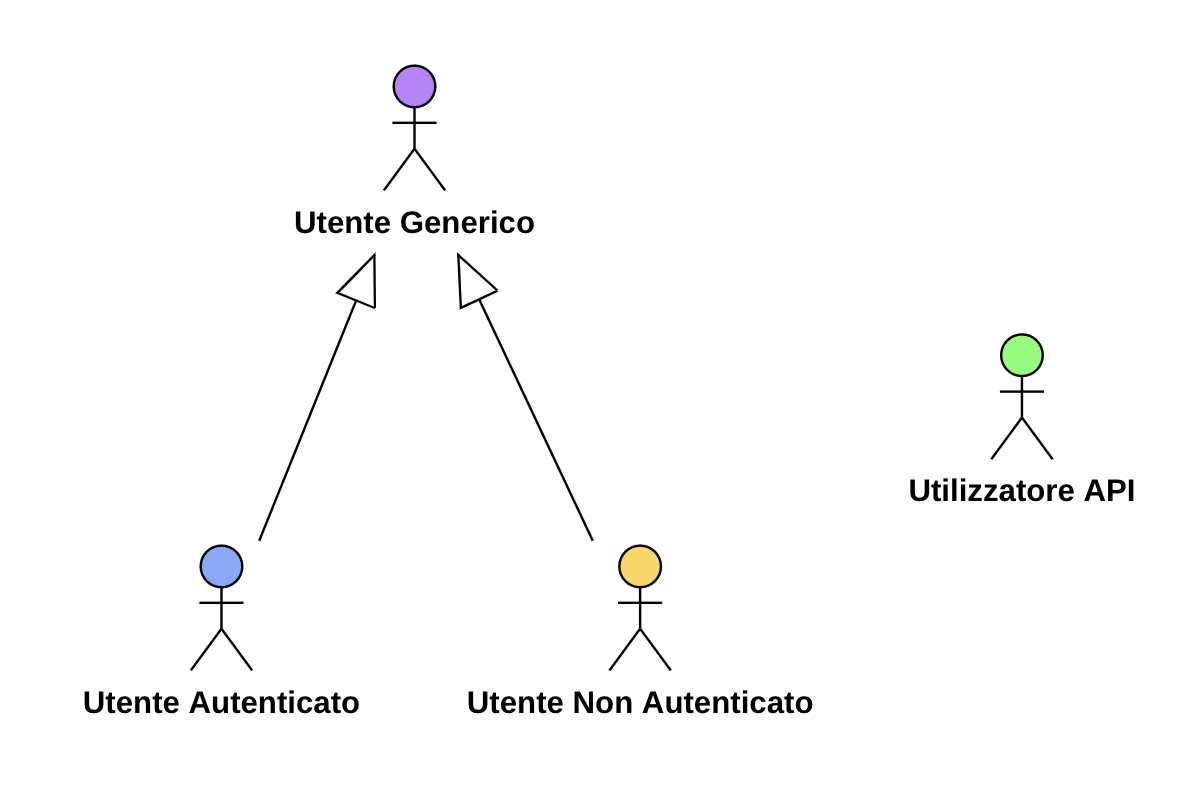
\includegraphics[scale=0.4]{src/img/attori_primari.png}
                \caption{Gerarchia degli attori primari}
            \end{figure}

            \paragraph*{Utente generico:} utente che non possiede un account \textit{MetaMask} e ha dunque possibilità di usufruire del servizio solo in lettura.

            \paragraph*{Utente non autenticato:} utente che possiede un account \textit{MetaMask} ma non è autenticato, dunque può usufruire del servizio solo in lettura o autenticarsi per poter effettuare pagamenti e rilasciare recensioni.

            \paragraph*{Utente autenticato:} utente che possiede un account \textit{MetaMask} e che è autenticato, dunque può effettuare pagamenti e rilasciare recensioni.

            \paragraph*{Utilizzatore API:} utente generico che utilizza l'\textit{API REST} per ottenere le recensioni, associate ad un indirizzo, in formato \textit{JSON}, senza passare per la \textit{web app}.

        \subsubsection{Attori secondari}
            \paragraph*{\textit{MetaMask}:} \textit{wallet}\glo \: di criptovalute usato per interagire con la \textit{blockchain} \textit{Ethereum}. Permette di accedere al proprio \textit{wallet} attraverso applicazione mobile o, come nel nostro caso, estensione per browser.

            \paragraph*{\textit{Infura}\glo:} backend \textit{Web3}\glo\:che offre servizi e strumenti per sviluppatori \textit{blockchain}; nel nostro caso sarà ciò che metterà in comunicazione \textit{web app} e \textit{API REST} con nodi\glo\:sulla \textit{blockchain}.

    \subsection{Elenco}

        \subsubsection{UC01 - Autenticazione}
        \label{UC01}

            \begin{figure}[H]
                \centering
                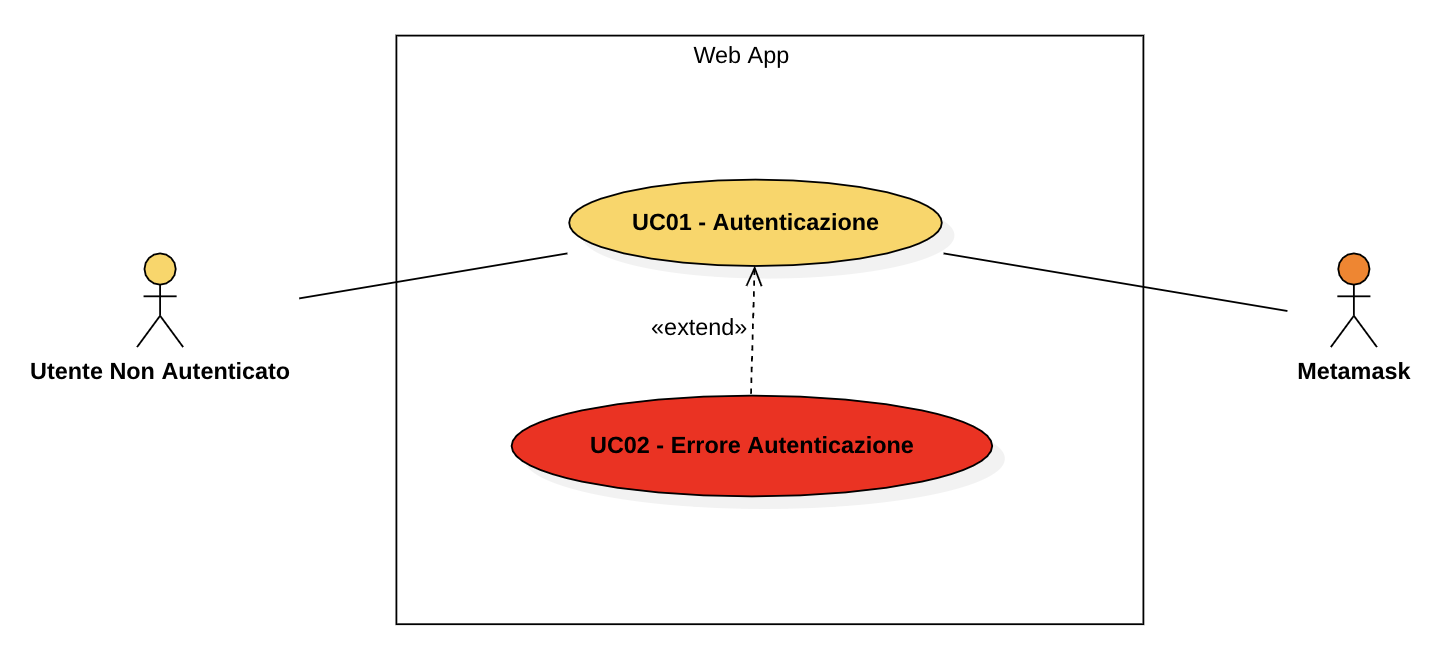
\includegraphics[scale=0.6]{src/img/UC01.png}
                \caption{UC01, UC02}
            \end{figure}

            \begin{table}[H]
                \centering
                \rowcolors{1}{pari_alt}{dispari_alt}
                \renewcommand{\arraystretch}{1.8}
                \renewcommand\tabularxcolumn[1]{m{#1}}
                \begin{tabularx}{0.9\textwidth} {
                    >{\hsize=.8\hsize\linewidth=\hsize}X
                    >{\hsize=1.2\hsize\linewidth=\hsize}X}
                    \hline
                    \textbf{Attore primario} & Utente non autenticato \\
                    \hline
                    \textbf{Attore secondario} & \textit{MetaMask} \\
                    \hline
                    \textbf{Precondizioni} & L'utente non è autenticato. \\
                    \hline
                    \textbf{Postcondizioni} & L'utente è autenticato. \\
                    \hline
                    \textbf{Scenario principale} & L'utente accede a \textit{MetaMask}. \\
                    \hline
                    \textbf{Estensioni} & Se l'accesso a \textit{MetaMask} non va a buon fine, si verifica \hyperref[UC02]{UC02}. \\
                    \hline
                \end{tabularx}
                \caption{UC01}
            \end{table}

            \subsubsection{UC02 - Errore Autenticazione}
            \label{UC02}
    
                \begin{table}[H]
                    \centering
                    \rowcolors{1}{pari_alt}{dispari_alt}
                    \renewcommand{\arraystretch}{1.8}
                    \renewcommand\tabularxcolumn[1]{m{#1}}
                    \begin{tabularx}{0.9\textwidth} {
                        >{\hsize=.8\hsize\linewidth=\hsize}X
                        >{\hsize=1.2\hsize\linewidth=\hsize}X}
                        \hline
                        \textbf{Attore primario} & Utente non autenticato \\
                        \hline
                        \textbf{Attore secondario} & \textit{MetaMask} \\
                        \hline
                        \textbf{Precondizioni} & L'utente sta tentando di autenticarsi. \\
                        \hline
                        \textbf{Postcondizioni} & L'operazione fallisce. \\
                        \hline
                        \textbf{Scenario principale} &
                            \begin{enumerate}
                                \item Si verificano problemi con l'accesso a \textit{MetaMask};
                                \item Viene mostrato un errore che informa l'utente del fallimento dell'operazione.
                            \end{enumerate} \\
                        \hline
                    \end{tabularx}
                    \caption{UC02}
                \end{table}

            \subsubsection{UC03 - Transazione}
            \label{UC03}
                \begin{figure}[H]
                    \centering
                    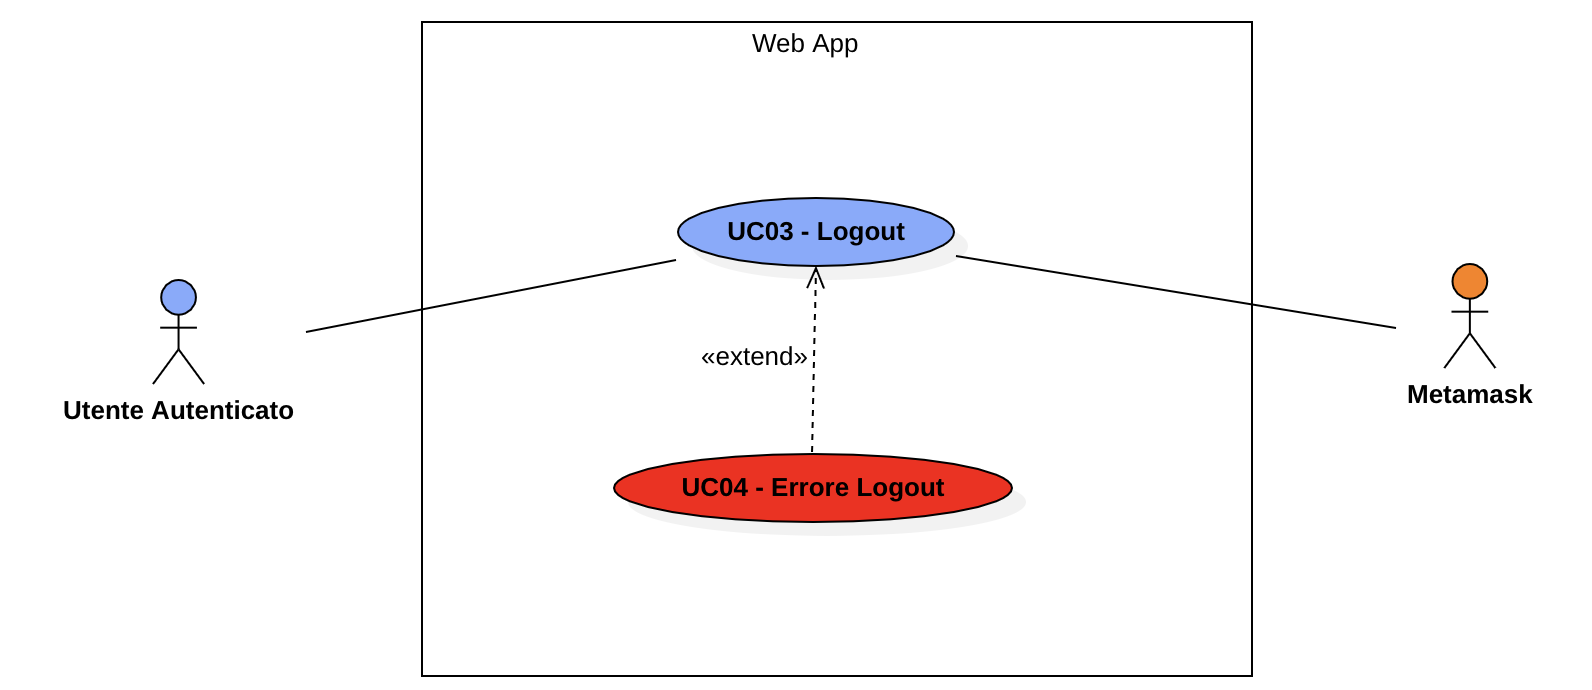
\includegraphics[scale=0.4]{src/img/UC03.png}
                    \caption{UC03}
                \end{figure}
    
                \begin{table}[H]
                    \centering
                    \rowcolors{1}{pari_alt}{dispari_alt}
                    \renewcommand{\arraystretch}{1.8}
                    \renewcommand\tabularxcolumn[1]{m{#1}}
                    \begin{tabularx}{0.9\textwidth} {
                        >{\hsize=.8\hsize\linewidth=\hsize}X
                        >{\hsize=1.2\hsize\linewidth=\hsize}X}
                        \hline
                        \textbf{Attore primario} & Utente autenticato \\
                        \hline
                        \textbf{Attore secondario} & \textit{MetaMask} e \textit{Infura} \\
                        \hline
                        \textbf{Precondizioni} & L'utente non ha ancora pagato. \\
                        \hline
                        \textbf{Postcondizioni} & L'utente ha completato il pagamento. \\
                        \hline
                        \textbf{Scenario principale} & L'utente effettua il pagamento verso un altro \textit{wallet}. \\
                        \hline
                    \end{tabularx}
                    \caption{UC03}
                \end{table}

            \subsubsection{UC04 - Errore Transazione}
            \label{UC04}

            \begin{figure}[H]
                \centering
                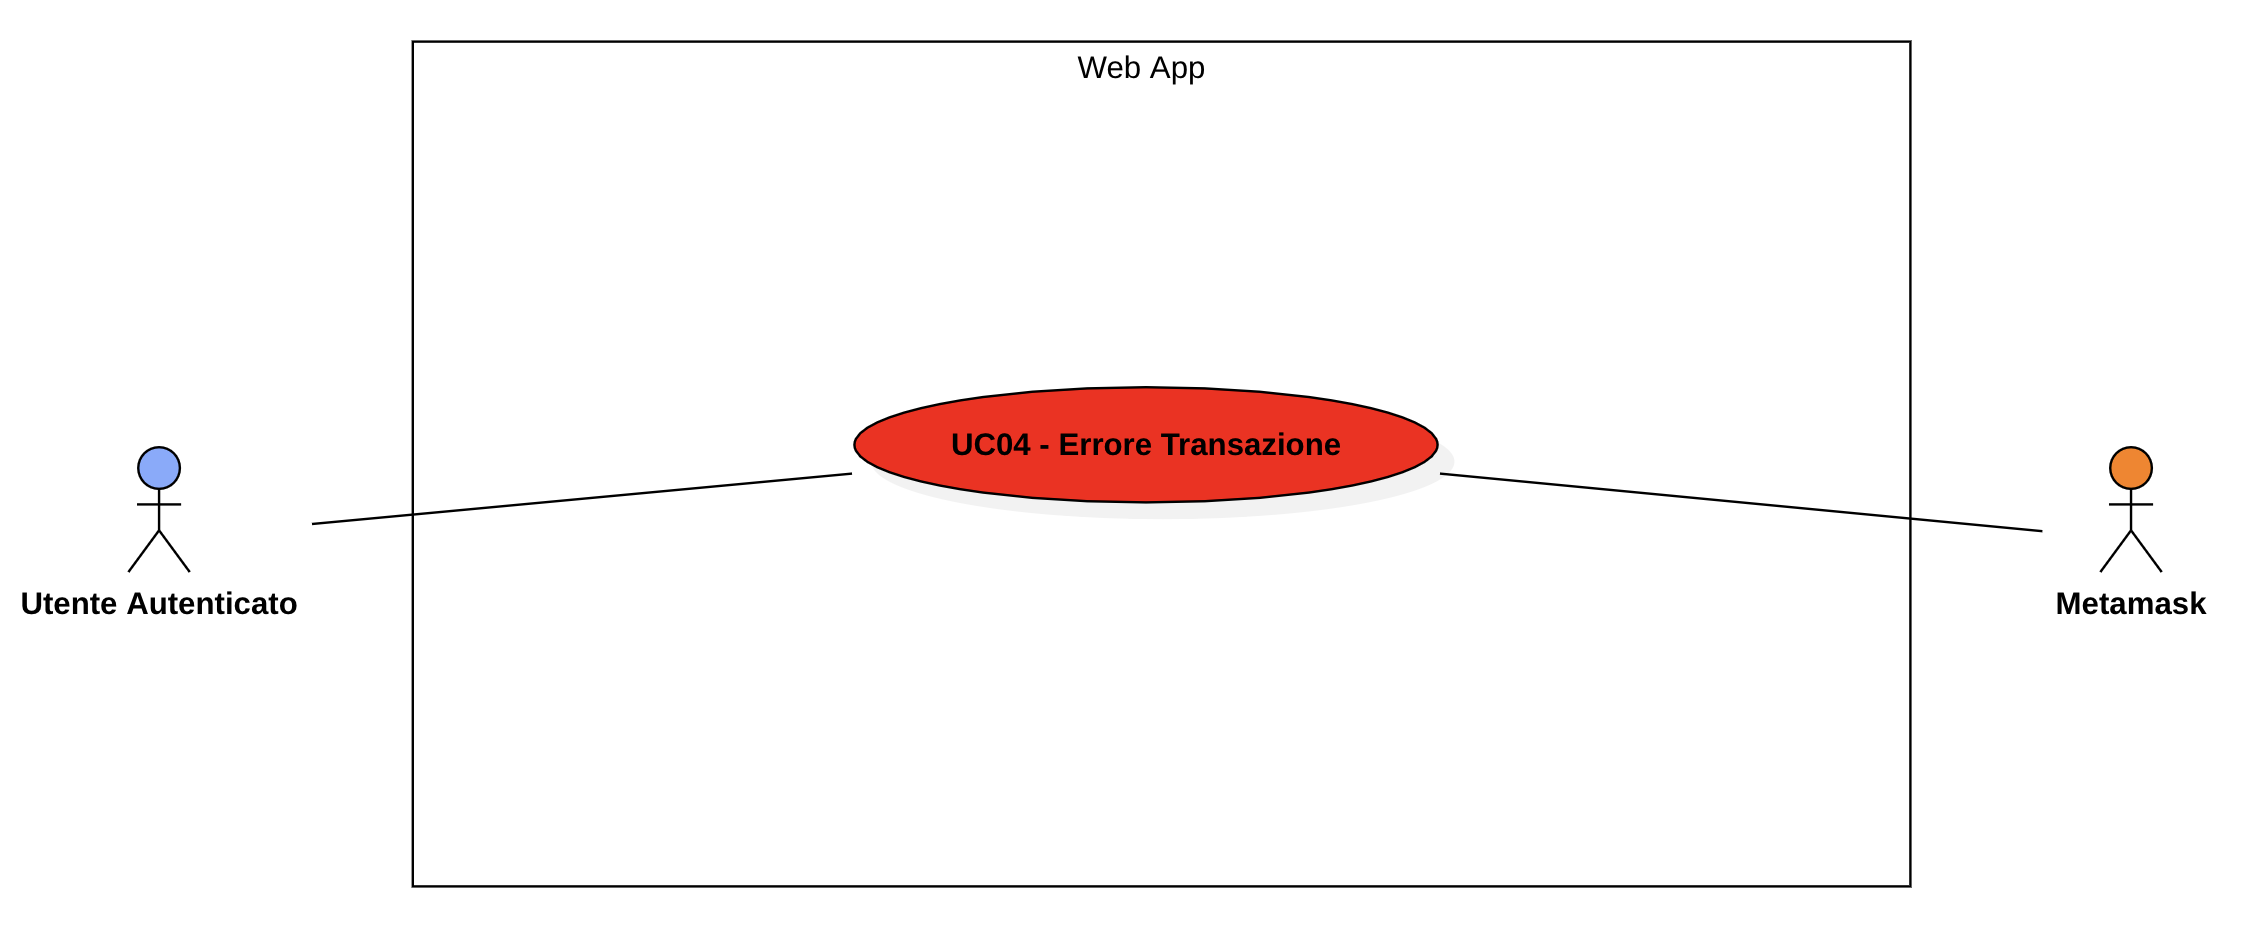
\includegraphics[scale=0.4]{src/img/UC04.png}
                \caption{UC04}
            \end{figure}
    
            \begin{table}[H]
                \centering
                \rowcolors{1}{pari_alt}{dispari_alt}
                \renewcommand{\arraystretch}{1.8}
                \renewcommand\tabularxcolumn[1]{m{#1}}
                \begin{tabularx}{0.9\textwidth} {
                    >{\hsize=.8\hsize\linewidth=\hsize}X
                    >{\hsize=1.2\hsize\linewidth=\hsize}X}
                    \hline
                    \textbf{Attore primario} & Utente autenticato \\
                    \hline
                    \textbf{Attore secondario} & \textit{MetaMask} \\
                    \hline
                    \textbf{Precondizioni} & L'utente sta tentando di effettuare un pagamento. \\
                    \hline
                    \textbf{Postcondizioni} & Il pagamento fallisce. \\
                    \hline
                    \textbf{Scenario principale} &
                    \begin{enumerate}
                        \item L'utente tenta di effettuare un pagamento che non va a buon fine;
                        \item Viene mostrato un errore che informa l'utente sul motivo del fallimento dell'operazione.
                        \item L'operazione viene annullata.
                    \end{enumerate} \\
                    \hline
                \end{tabularx}
                \caption{UC04}
            \end{table}

        \subsubsection{UC05 - Rilascio Recensione}
        \label{UC05}

            \begin{figure}[H]
                \centering
                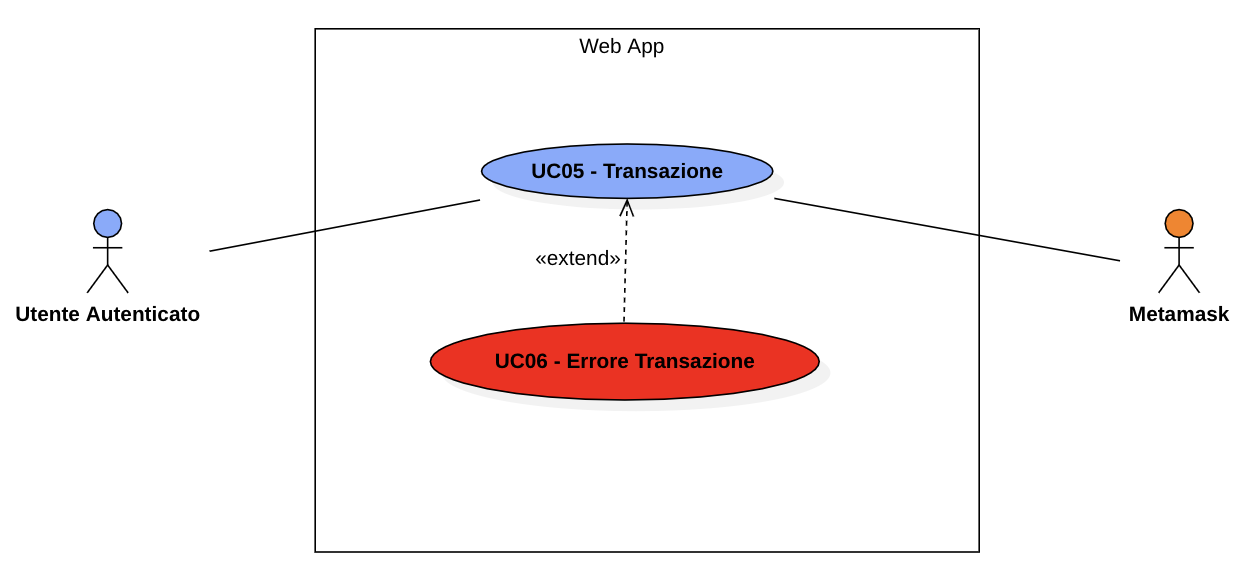
\includegraphics[scale=0.4]{src/img/UC05.png}
                \caption{UC05, UC06}
            \end{figure}

            \begin{figure}[H]
                \centering
                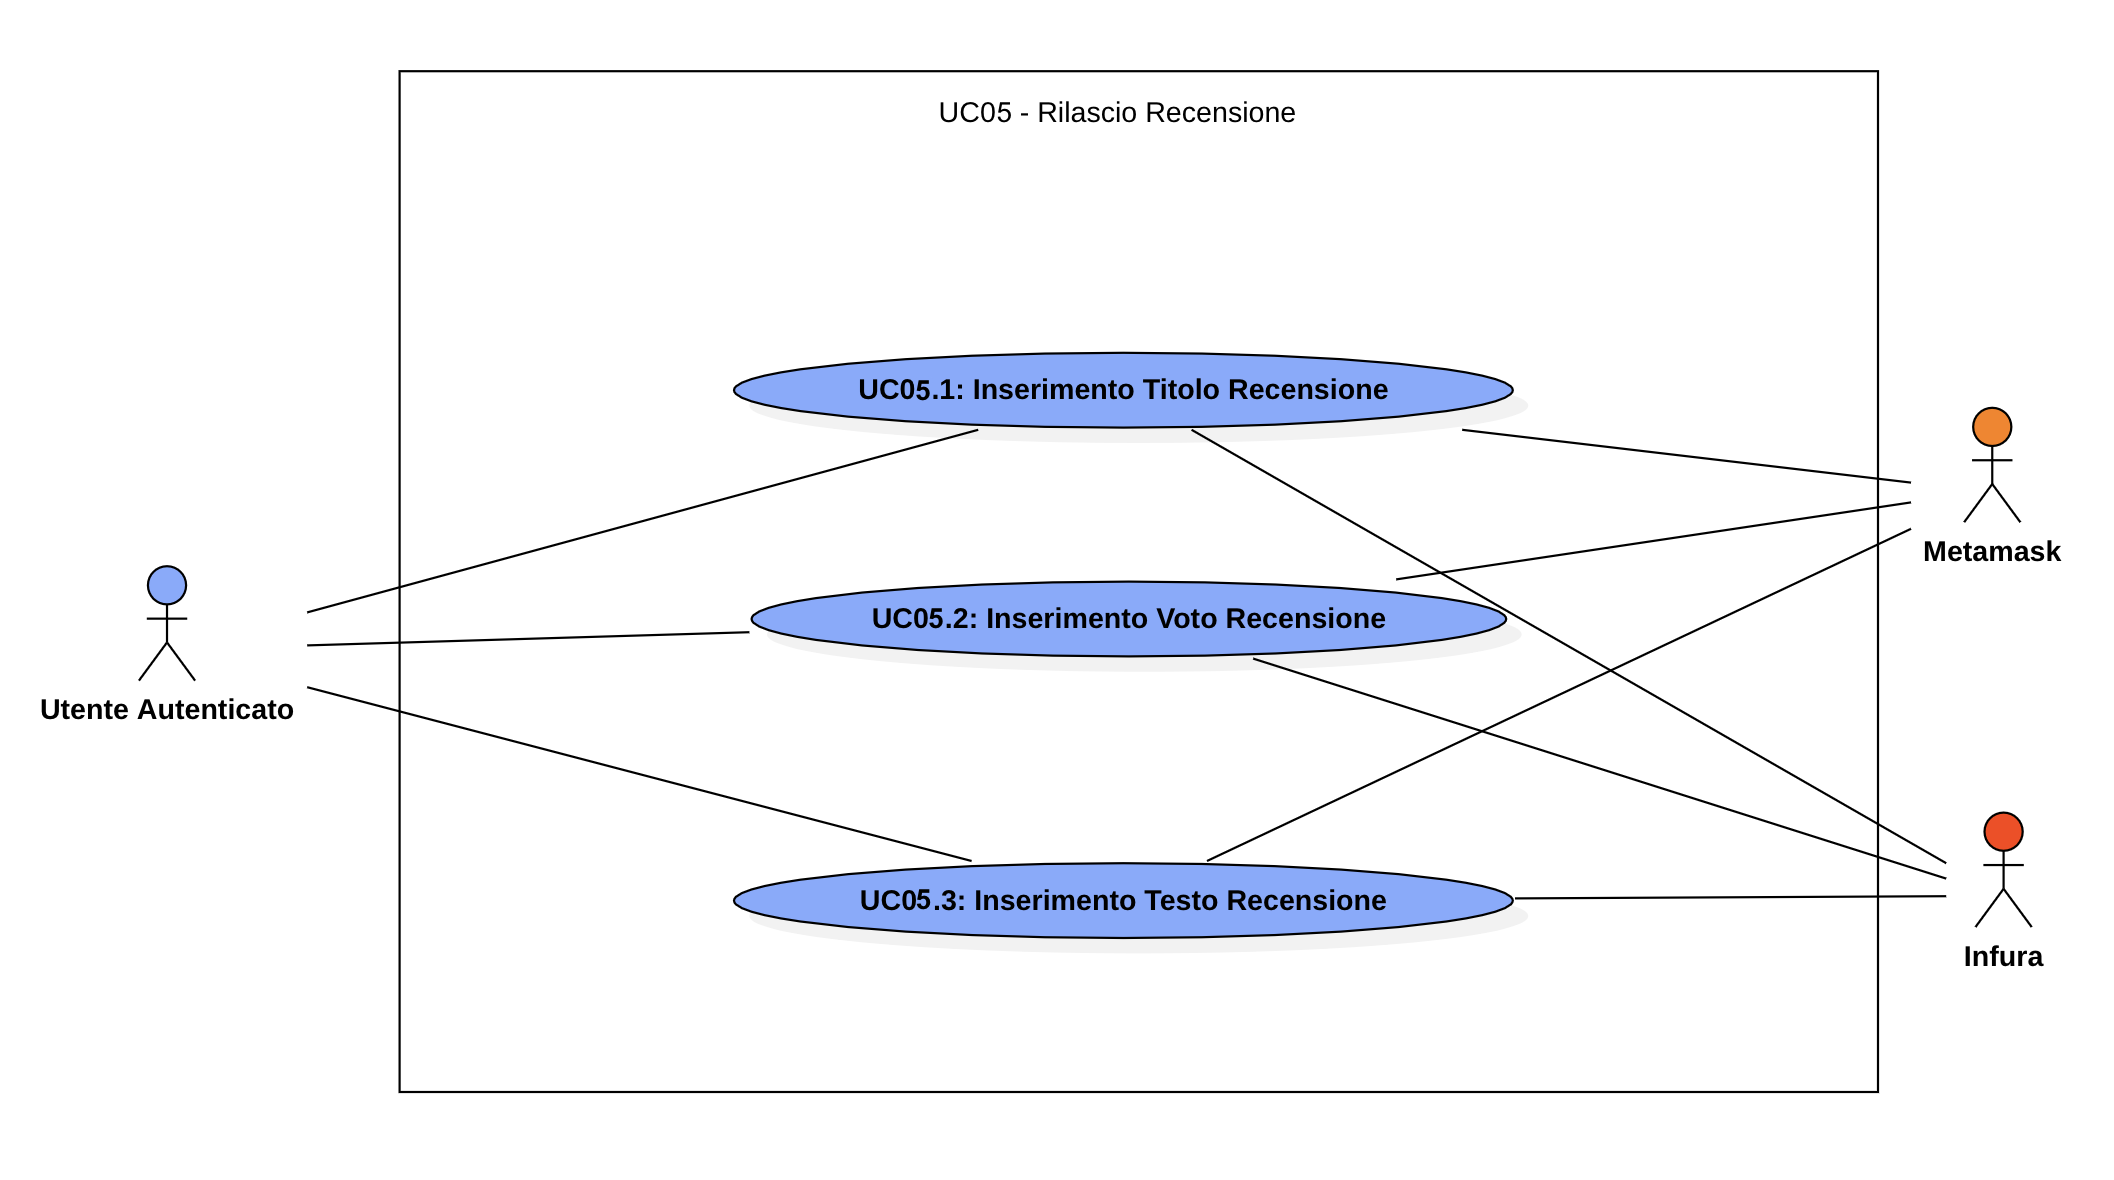
\includegraphics[scale=0.4]{src/img/UC05.X.png}
                \caption{UC05.1, UC05.2, UC05.3}
            \end{figure}

            \begin{table}[H]
                \centering
                \rowcolors{1}{pari_alt}{dispari_alt}
                \renewcommand{\arraystretch}{1.8}
                \renewcommand\tabularxcolumn[1]{m{#1}}
                \begin{tabularx}{0.9\textwidth}{
                    >{\hsize=.8\hsize\linewidth=\hsize}X
                    >{\hsize=1.2\hsize\linewidth=\hsize}X}
                    \hline
                    \textbf{Attore primario} & Utente autenticato \\
                    \hline
                    \textbf{Attore secondario} & \textit{Infura}, \textit{MetaMask} \\
                    \hline
                    \textbf{Precondizioni} &
                        \begin{itemize}
                            \item L'utente è autenticato;
                            \item l'utente ha effettuato almeno un acquisto;
                            \item l'utente ha acquisti non recensiti.
                        \end{itemize} \\
                    \hline
                    \textbf{Postcondizioni} & L'utente ha effettuato una recensione sull'acquisto. \\
                    \hline
                    \textbf{Scenario principale} &
                    L'utente seleziona un pagamento da associare alla recensione.\\
                    \hline
                    \textbf{Estensioni} & Se il rilascio di una recensione non va a buon fine, si verifica \hyperref[UC05]{UC05}. \\
                    \hline
                \end{tabularx}
                \caption{UC05}
            \end{table}

            \subsubsection{UC05.1 - Inserimento Titolo Recensione}
            \label{UC05.1}

                \begin{table}[H]
                    \centering
                    \rowcolors{1}{pari_alt}{dispari_alt}
                    \renewcommand{\arraystretch}{1.8}
                    \renewcommand\tabularxcolumn[1]{m{#1}}
                    \begin{tabularx}{0.9\textwidth}{
                        >{\hsize=.8\hsize\linewidth=\hsize}X
                        >{\hsize=1.2\hsize\linewidth=\hsize}X}
                        \hline
                        \textbf{Attore primario} & Utente autenticato \\
                        \hline
                        \textbf{Attore secondario} & \textit{Infura}, \textit{MetaMask} \\
                        \hline
                        \textbf{Precondizioni} &
                            \begin{itemize}
                                \item L'utente è autenticato;
                                \item l'utente ha effettuato almeno un acquisto;
                                \item l'utente ha acquisti non recensiti.
                            \end{itemize} \\
                        \hline
                        \textbf{Postcondizioni} & La recensione ha un titolo inserito dall'utente. \\
                        \hline
                        \textbf{Scenario principale} &
                        L'utente ha inserito un titolo per la recensione. \\
                        \hline
                        \textbf{Estensioni} & Se il rilascio di una recensione non va a buon fine, si verifica \hyperref[UC06]{UC06}. \\
                        \hline
                    \end{tabularx}
                    \caption{UC05.1}
                \end{table}

            \subsubsection{UC05.2 - Inserimento Voto Recensione}
            \label{UC05.2}

                \begin{table}[H]
                    \centering
                    \rowcolors{1}{pari_alt}{dispari_alt}
                    \renewcommand{\arraystretch}{1.8}
                    \renewcommand\tabularxcolumn[1]{m{#1}}
                    \begin{tabularx}{0.9\textwidth}{
                        >{\hsize=.8\hsize\linewidth=\hsize}X
                        >{\hsize=1.2\hsize\linewidth=\hsize}X}
                        \hline
                        \textbf{Attore primario} & Utente autenticato \\
                        \hline
                        \textbf{Attore secondario} & \textit{Infura}, \textit{MetaMask} \\
                        \hline
                        \textbf{Precondizioni} &
                            \begin{itemize}
                                \item L'utente è autenticato;
                                \item l'utente ha effettuato almeno un acquisto;
                                \item l'utente ha acquisti non recensiti.
                            \end{itemize} \\
                        \hline
                        \textbf{Postcondizioni} & La recensione ha un voto inserito dall'utente. \\
                        \hline
                        \textbf{Scenario principale} &
                        L'utente ha inserito un voto per la recensione. \\
                        \hline
                        \textbf{Estensioni} & Se il rilascio di una recensione non va a buon fine, si verifica \hyperref[UC06]{UC06}. \\
                        \hline
                    \end{tabularx}
                    \caption{UC05.2}
                \end{table}

            \subsubsection{UC05.3 - Inserimento Testo Recensione}
            \label{UC05.3}

                \begin{table}[H]
                    \centering
                    \rowcolors{1}{pari_alt}{dispari_alt}
                    \renewcommand{\arraystretch}{1.8}
                    \renewcommand\tabularxcolumn[1]{m{#1}}
                    \begin{tabularx}{0.9\textwidth}{
                        >{\hsize=.8\hsize\linewidth=\hsize}X
                        >{\hsize=1.2\hsize\linewidth=\hsize}X}
                        \hline
                        \textbf{Attore primario} & Utente autenticato \\
                        \hline
                        \textbf{Attore secondario} & \textit{Infura}, \textit{MetaMask} \\
                        \hline
                        \textbf{Precondizioni} &
                            \begin{itemize}
                                \item L'utente è autenticato;
                                \item l'utente ha effettuato almeno un acquisto;
                                \item l'utente ha acquisti non recensiti.
                            \end{itemize} \\
                        \hline
                        \textbf{Postcondizioni} & La recensione ha un testo inserito dall'utente. \\
                        \hline
                        \textbf{Scenario principale} &
                        L'utente ha inserito un testo per la recensione. \\
                        \hline
                        \textbf{Estensioni} & Se il rilascio di una recensione non va a buon fine, si verifica \hyperref[UC06]{UC06}. \\
                        \hline
                    \end{tabularx}
                    \caption{UC05.3}
                \end{table}

        \subsubsection{UC06 - Errore Rilascio Recensione}
        \label{UC06}

            \begin{table}[H]
                \centering
                \rowcolors{1}{pari_alt}{dispari_alt}
                \renewcommand{\arraystretch}{1.8}
                \renewcommand\tabularxcolumn[1]{m{#1}}
                \begin{tabularx}{0.9\textwidth} {
                    >{\hsize=.8\hsize\linewidth=\hsize}X
                    >{\hsize=1.2\hsize\linewidth=\hsize}X}
                    \hline
                    \textbf{Attore primario} & Utente autenticato \\
                    \hline
                    \textbf{Attore secondario} & \textit{MetaMask} \\
                    \hline
                    \textbf{Precondizioni} & L'utente vuole rilasciare una recensione. \\
                    \hline
                    \textbf{Postcondizioni} & L'operazione fallisce. \\
                    \hline
                    \textbf{Scenario principale} &
                        \begin{enumerate}
                            \item L'utente rilascia una recensione che rispetta un formato valido, ovvero non viola i seguenti vincoli:
                            \begin{itemize}
                                \item titolo: non vuoto e non superiore a 50 caratteri;
                                \item voto: non vuoto e compreso tra 1 e 5;
                                \item testo: non vuoto e non superiore a 500 caratteri;
                            \end{itemize}
                            \item Viene mostrato un errore che informa l'utente sulla motivazione e si termina l'attuale operazione.
                        \end{enumerate} \\
                    \hline
                \end{tabularx}
                \caption{UC06}
            \end{table}

        \subsubsection{UC07 - Ricerca Recensioni}
        \label{UC07}

            \begin{figure}[H]
                \centering
                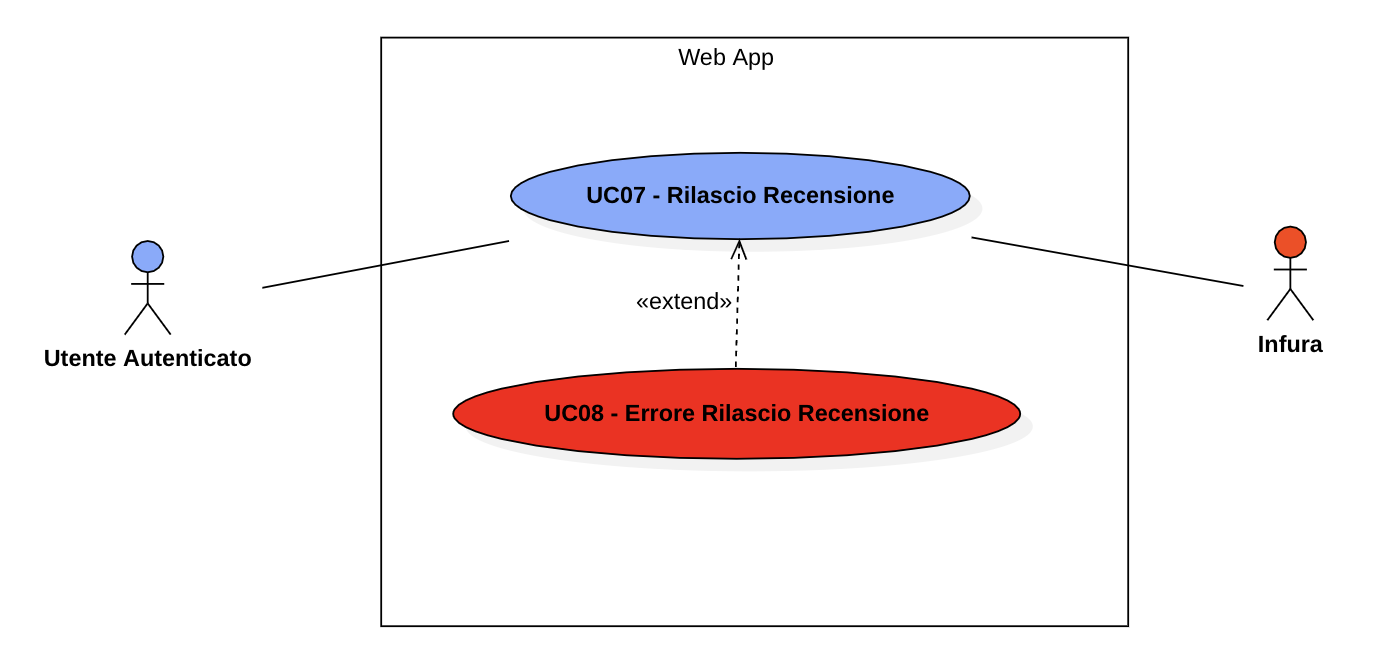
\includegraphics[scale=0.6]{src/img/UC07.png}
                \caption{UC07, UC10}
                \includegraphics[scale=0.4]{src/img/UC07.x.png}
                \caption{UC07.1 - UC07.6}
            \end{figure}

            \begin{table}[H]
                \centering
                \rowcolors{1}{pari_alt}{dispari_alt}
                \renewcommand{\arraystretch}{1.8}
                \renewcommand\tabularxcolumn[1]{m{#1}}
                \begin{tabularx}{0.9\textwidth} {
                    >{\hsize=.8\hsize\linewidth=\hsize}X
                    >{\hsize=1.2\hsize\linewidth=\hsize}X}
                    \hline
                    \textbf{Attore primario} & Utente generico \\
                    \hline
                    \textbf{Attore secondario} & Infura \\
                    \hline
                    \textbf{Precondizioni} & L'utente vuole ricercare le recensioni di un dato indirizzo. \\
                    \hline
                    \textbf{Postcondizioni} & L'utente ha ottenuto le informazioni disponibili. \\
                    \hline
                    \textbf{Scenario principale} & L'utente effettua la ricerca secondo alcuni criteri. \\
                    \hline
                    \textbf{Estensioni} & Se l'operazione non va a buon fine, si verifica \hyperref[UC10]{UC10}. \\
                    \hline
                \end{tabularx}
                \caption{UC07}
            \end{table}

        \subsubsection{UC07.1 - Ricerca Recensioni per indirizzo}
        \label{UC07.1}

            \begin{table}[H]
                \centering
                \rowcolors{1}{pari_alt}{dispari_alt}
                \renewcommand{\arraystretch}{1.8}
                \renewcommand\tabularxcolumn[1]{m{#1}}
                \begin{tabularx}{0.9\textwidth} {
                    >{\hsize=.8\hsize\linewidth=\hsize}X
                    >{\hsize=1.2\hsize\linewidth=\hsize}X}
                    \hline
                    \textbf{Attore primario} & Utente generico \\
                    \hline
                    \textbf{Attore secondario} & Infura \\
                    \hline
                    \textbf{Precondizioni} & L'utente conosce l'indirizzo di cui cercare le recensioni. \\
                    \hline
                    \textbf{Postcondizioni} & L'utente ha ottenuto le informazioni. \\
                    \hline
                    \textbf{Scenario principale} & L'utente ricerca le recensioni inserendo l'indirizzo di cui vuole ottenere informazioni.\\
                    \hline
                    \textbf{Estensioni} & Se l'operazione non va a buon fine, si verifica \hyperref[UC10]{UC10}. \\
                    \hline
                \end{tabularx}
                \caption{UC07.1}
            \end{table}

        \subsubsection{UC07.2 - Ricerca Recensioni per autore}
        \label{UC07.2}

            \begin{table}[H]
                \centering
                \rowcolors{1}{pari_alt}{dispari_alt}
                \renewcommand{\arraystretch}{1.8}
                \renewcommand\tabularxcolumn[1]{m{#1}}
                \begin{tabularx}{0.9\textwidth} {
                    >{\hsize=.8\hsize\linewidth=\hsize}X
                    >{\hsize=1.2\hsize\linewidth=\hsize}X}
                    \hline
                    \textbf{Attore primario} & Utente generico \\
                    \hline
                    \textbf{Attore secondario} & Infura \\
                    \hline
                    \textbf{Precondizioni} & L'utente è interessato alle recensioni rilasciate da un particolare utente. \\
                    \hline
                    \textbf{Postcondizioni} & L'utente ha ottenuto le informazioni che cercava. \\
                    \hline
                    \textbf{Scenario principale} & L'utente ricerca delle recensioni specificando che l'indirizzo inserito fa riferimento all'autore.\\
                    \hline
                    \textbf{Estensioni} & Se l'operazione non va a buon fine, si verifica \hyperref[UC10]{UC10}. \\
                    \hline
                \end{tabularx}
                \caption{UC07.2}
            \end{table}

        \subsubsection{UC07.3 - Ricerca Recensioni per destinatario}
        \label{UC07.3}

            \begin{table}[H]
                \centering
                \rowcolors{1}{pari_alt}{dispari_alt}
                \renewcommand{\arraystretch}{1.8}
                \renewcommand\tabularxcolumn[1]{m{#1}}
                \begin{tabularx}{0.9\textwidth} {
                    >{\hsize=.8\hsize\linewidth=\hsize}X
                    >{\hsize=1.2\hsize\linewidth=\hsize}X}
                    \hline
                    \textbf{Attore primario} & Utente generico \\
                    \hline
                    \textbf{Attore secondario} & Infura \\
                    \hline
                    \textbf{Precondizioni} & L'utente è interessato alle recensioni ricevute da un particolare utente. \\
                    \hline
                    \textbf{Postcondizioni} & L'utente ha ottenuto le informazioni che cercava. \\
                    \hline
                    \textbf{Scenario principale} & L'utente ricerca delle recensioni specificando che l'indirizzo inserito fa riferimento al destinatario.\\
                    \hline
                    \textbf{Estensioni} & Se l'operazione non va a buon fine, si verifica \hyperref[UC10]{UC10}. \\
                    \hline
                \end{tabularx}
                \caption{UC07.3}
            \end{table}

        \subsubsection{UC07.4 - Ricerca Recensioni per voto}
        \label{UC07.4}

            \begin{table}[H]
                \centering
                \rowcolors{1}{pari_alt}{dispari_alt}
                \renewcommand{\arraystretch}{1.8}
                \renewcommand\tabularxcolumn[1]{m{#1}}
                \begin{tabularx}{0.9\textwidth} {
                    >{\hsize=.8\hsize\linewidth=\hsize}X
                    >{\hsize=1.2\hsize\linewidth=\hsize}X}
                    \hline
                    \textbf{Attore primario} & Utente generico \\
                    \hline
                    \textbf{Attore secondario} & Infura \\
                    \hline
                    \textbf{Precondizioni} & L'utente è interessato alle recensioni con un particolare voto \\
                    \hline
                    \textbf{Postcondizioni} & L'utente ha ottenuto le informazioni che cercava. \\
                    \hline
                    \textbf{Scenario principale} & L'utente ricerca delle recensioni specificando il voto per cui filtrarle.\\
                    \hline
                    \textbf{Estensioni} & Se l'operazione non va a buon fine, si verifica \hyperref[UC10]{UC10}. \\
                    \hline
                \end{tabularx}
                \caption{UC07.4}
            \end{table}

        \subsubsection{UC07.5 - Ricerca Recensioni per titolo}
        \label{UC07.5}

            \begin{table}[H]
                \centering
                \rowcolors{1}{pari_alt}{dispari_alt}
                \renewcommand{\arraystretch}{1.8}
                \renewcommand\tabularxcolumn[1]{m{#1}}
                \begin{tabularx}{0.9\textwidth} {
                    >{\hsize=.8\hsize\linewidth=\hsize}X
                    >{\hsize=1.2\hsize\linewidth=\hsize}X}
                    \hline
                    \textbf{Attore primario} & Utente generico \\
                    \hline
                    \textbf{Attore secondario} & Infura \\
                    \hline
                    \textbf{Precondizioni} & L'utente è interessato alle recensioni con un particolare titolo \\
                    \hline
                    \textbf{Postcondizioni} & L'utente ha ottenuto le informazioni che cercava. \\
                    \hline
                    \textbf{Scenario principale} & L'utente ricerca delle recensioni specificando il titolo per cui filtrarle.\\
                    \hline
                    \textbf{Estensioni} & Se l'operazione non va a buon fine, si verifica \hyperref[UC10]{UC10}. \\
                    \hline
                \end{tabularx}
                \caption{UC07.5}
            \end{table}

        \subsubsection{UC07.6 - Ricerca Recensioni per data}
        \label{UC07.6}

            \begin{table}[H]
                \centering
                \rowcolors{1}{pari_alt}{dispari_alt}
                \renewcommand{\arraystretch}{1.8}
                \renewcommand\tabularxcolumn[1]{m{#1}}
                \begin{tabularx}{0.9\textwidth} {
                    >{\hsize=.8\hsize\linewidth=\hsize}X
                    >{\hsize=1.2\hsize\linewidth=\hsize}X}
                    \hline
                    \textbf{Attore primario} & Utente generico \\
                    \hline
                    \textbf{Attore secondario} & Infura \\
                    \hline
                    \textbf{Precondizioni} & L'utente è interessato alle recensioni di uno specifico periodo \\
                    \hline
                    \textbf{Postcondizioni} & L'utente ha ottenuto le informazioni che cercava. \\
                    \hline
                    \textbf{Scenario principale} & L'utente ricerca delle recensioni specificando la data di riferimento per cui filtrarle.\\
                    \hline
                    \textbf{Estensioni} & Se l'operazione non va a buon fine, si verifica \hyperref[UC10]{UC10}. \\
                    \hline
                \end{tabularx}
                \caption{UC07.6}
            \end{table}

        \subsubsection{UC08 - Ricerca Recensioni Rilasciate}
        \label{UC08}

            \begin{figure}[H]
                \centering
                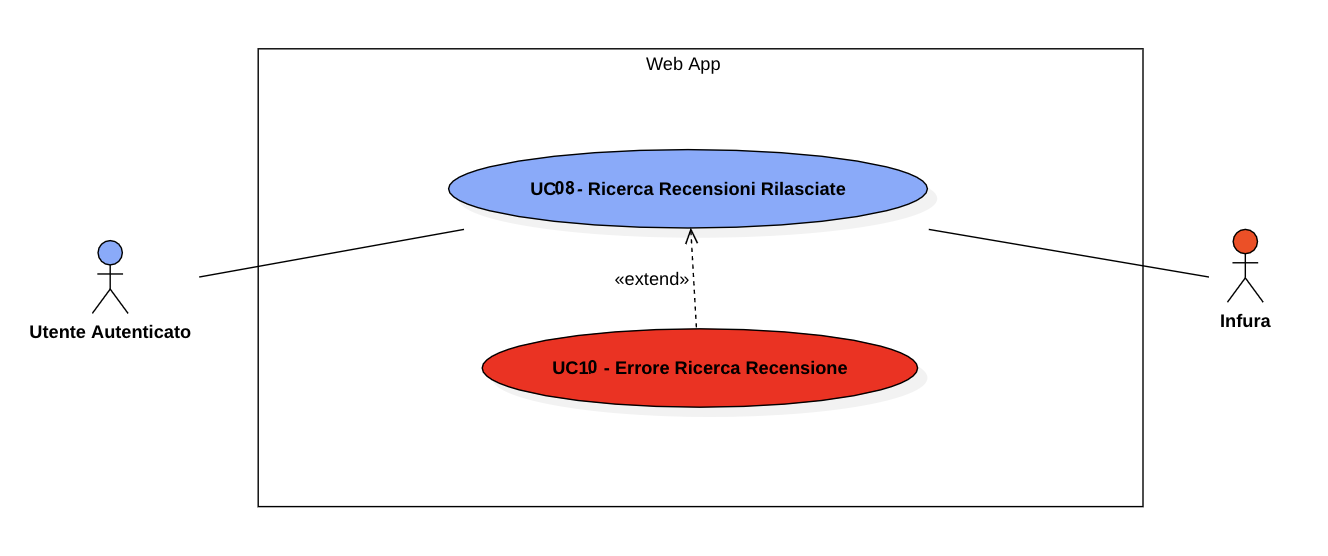
\includegraphics[scale=0.6]{src/img/UC08.png}
                \caption{UC08, UC10}
            \end{figure}

            \begin{table}[H]
                \centering
                \rowcolors{1}{pari_alt}{dispari_alt}
                \renewcommand{\arraystretch}{1.8}
                \renewcommand\tabularxcolumn[1]{m{#1}}
                \begin{tabularx}{0.9\textwidth} {
                    >{\hsize=.8\hsize\linewidth=\hsize}X
                    >{\hsize=1.2\hsize\linewidth=\hsize}X}
                    \hline
                    \textbf{Attore primario} & Utente autenticato \\
                    \hline
                    \textbf{Attore secondario} & Infura \\
                    \hline
                    \textbf{Precondizioni} & L'utente vuole ricercare le recensioni che ha rilasciato. \\
                    \hline
                    \textbf{Postcondizioni} & L'utente ottiene le informazioni sulle proprie recensioni.\\
                    \hline
                    \textbf{Scenario principale} & L'utente richiede la la lista delle recensioni che ha rilasciato come autore.\\
                    \hline
                    \textbf{Estensioni} & Se l'operazione non va a buon fine, si verifica \hyperref[UC10]{UC10}. \\
                    \hline
                \end{tabularx}
                \caption{UC08}
            \end{table}

        \subsubsection{UC09 - Ricerca Recensioni Ricevute}
        \label{UC09}

            \begin{figure}[H]
                \centering
                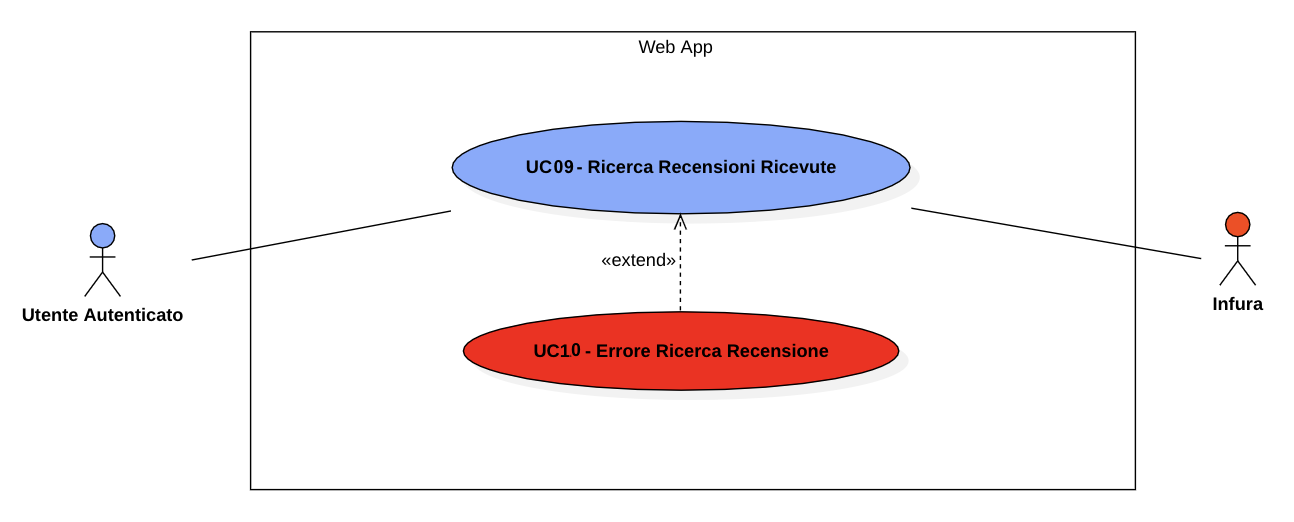
\includegraphics[scale=0.6]{src/img/UC09.png}
                \caption{UC09, UC11}
            \end{figure}

            \begin{table}[H]
                \centering
                \rowcolors{1}{pari_alt}{dispari_alt}
                \renewcommand{\arraystretch}{1.8}
                \renewcommand\tabularxcolumn[1]{m{#1}}
                \begin{tabularx}{0.9\textwidth} {
                    >{\hsize=.8\hsize\linewidth=\hsize}X
                    >{\hsize=1.2\hsize\linewidth=\hsize}X}
                    \hline
                    \textbf{Attore primario} & Utente autenticato \\
                    \hline
                    \textbf{Attore secondario} & Infura \\
                    \hline
                    \textbf{Precondizioni} & L'utente vuole ricercare le recensioni che ha ricevuto. \\
                    \hline
                    \textbf{Postcondizioni} & L'utente ottiene le informazioni sulle proprie recensioni.\\
                    \hline
                    \textbf{Scenario principale} & L'utente richiede la la lista delle recensioni che ha ricevuto come attività.\\
                    \hline
                    \textbf{Estensioni} & Se l'operazione non va a buon fine, si verifica \hyperref[UC10]{UC10}. \\
                    \hline
                \end{tabularx}
                \caption{UC09}
            \end{table}

        \subsubsection{UC10 - Errore Ricerca Recensioni}
        \label{UC10}

            \begin{table}[H]
                \centering
                \rowcolors{1}{pari_alt}{dispari_alt}
                \renewcommand{\arraystretch}{1.8}
                \renewcommand\tabularxcolumn[1]{m{#1}}
                \begin{tabularx}{0.9\textwidth} {
                    >{\hsize=.8\hsize\linewidth=\hsize}X
                    >{\hsize=1.2\hsize\linewidth=\hsize}X}
                    \hline
                    \textbf{Attori primari} & Utente generico. \\
                    \hline
                    \textbf{Attore secondario} & \textit{Infura} \\
                    \hline
                    \textbf{Precondizioni} & L'utente ricerca le recensioni collegate ad un indirizzo. \\
                    \hline
                    \textbf{Postcondizioni} & La ricerca fallisce. \\
                    \hline
                    \textbf{Scenario principale} & La ricerca effettuata dall'utente fallisce ,e viene visualizzato un errore, per i seguenti motivi:
                    \begin{itemize}
                        \item tutti i campi sono vuoti;
                        \item inserimento di un indirizzo wallet non valido;
                        \item non sono presenti recensioni con il voto inserito dall'utente;
                        \item inserimento di un titolo inesistente;
                        \item non esistono recensioni rilasciate nella data inserita dall'utente.
                    \end{itemize} \\
                    \hline
                \end{tabularx}
                \caption{UC10}
            \end{table}

        \subsubsection{UC11 - Visualizzazione Lista Recensioni}
        \label{UC11}

            \begin{figure}[H]
                \centering
                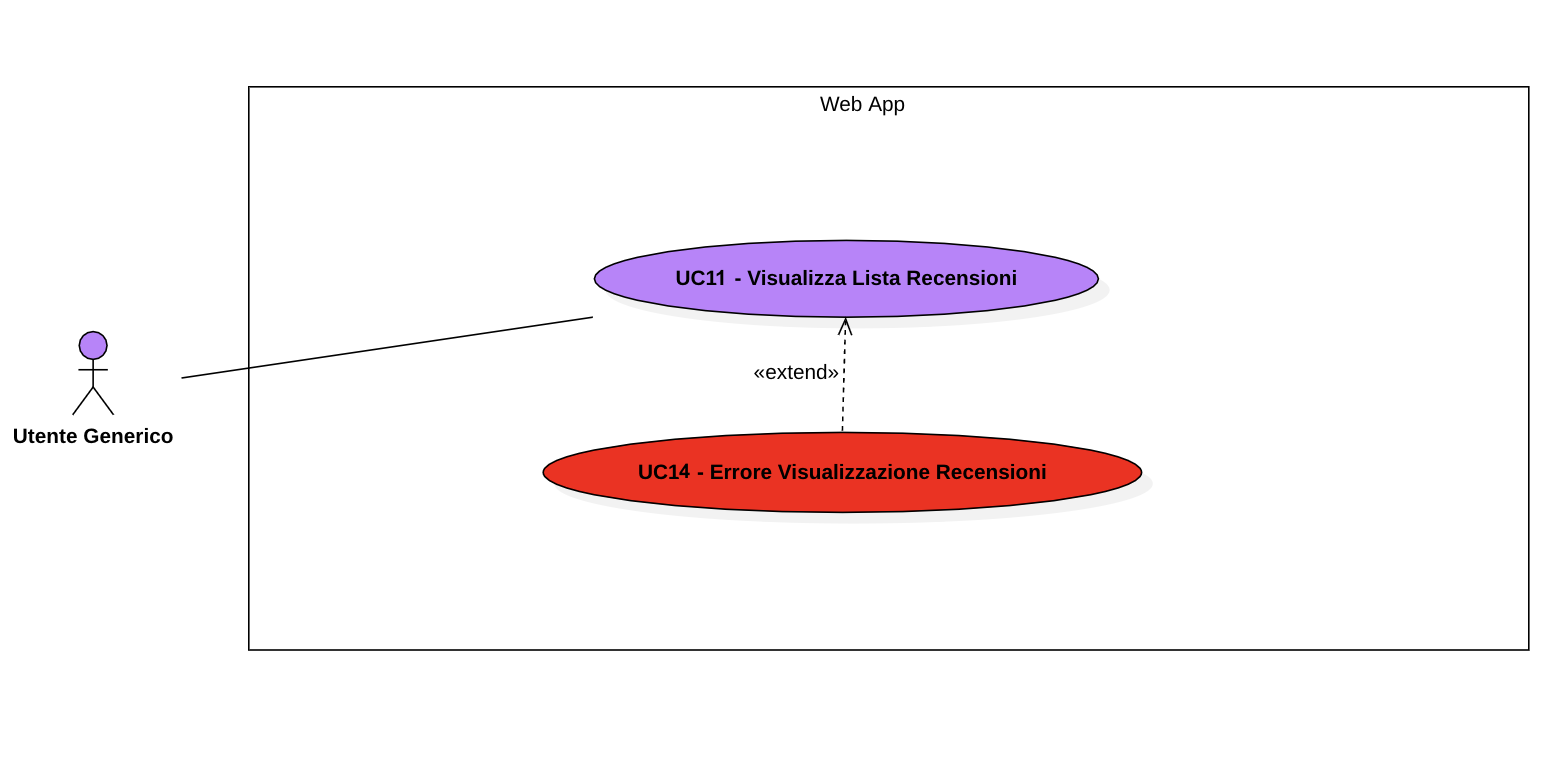
\includegraphics[scale=0.6]{src/img/UC11.png}
                \caption{UC11, 14}
            \end{figure}

            \begin{table}[H]
                \centering
                \rowcolors{1}{pari_alt}{dispari_alt}
                \renewcommand{\arraystretch}{1.8}
                \renewcommand\tabularxcolumn[1]{m{#1}}
                \begin{tabularx}{0.9\textwidth} {
                    >{\hsize=.8\hsize\linewidth=\hsize}X
                    >{\hsize=1.2\hsize\linewidth=\hsize}X}
                    \hline
                    \textbf{Attore primario} & Utente generico \\
                    \hline
                    \textbf{Precondizioni} & L'utente ha effettuato una ricerca delle recensioni, che è andata a buon fine. \\
                    \hline
                    \textbf{Postcondizioni} & L'utente visualizza le recensioni associate ad una ricerca. \\
                    \hline
                    \textbf{Scenario principale} & Viene visualizzata una lista di recensioni corrispondenti. \\
                    \hline
                    \textbf{Estensioni} & Se l'operazione non va a buon fine, si verifica \hyperref[UC16]{UC16}. \\
                    \hline
                \end{tabularx}
                \caption{UC11}
            \end{table}

        \subsubsection{UC11.1 - Visualizzazione Singola Recensione}
        \label{UC11.1}

            \begin{figure}[H]
                \centering
                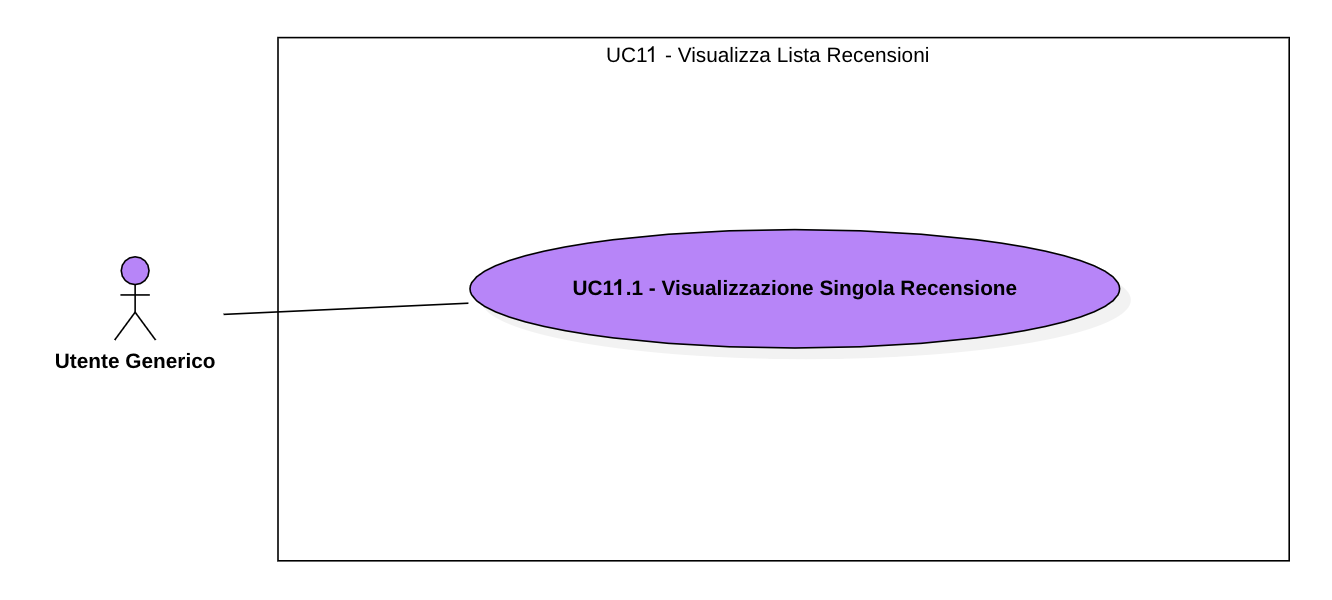
\includegraphics[scale=0.6]{src/img/UC11.1.png}
                \caption{UC11.1}
                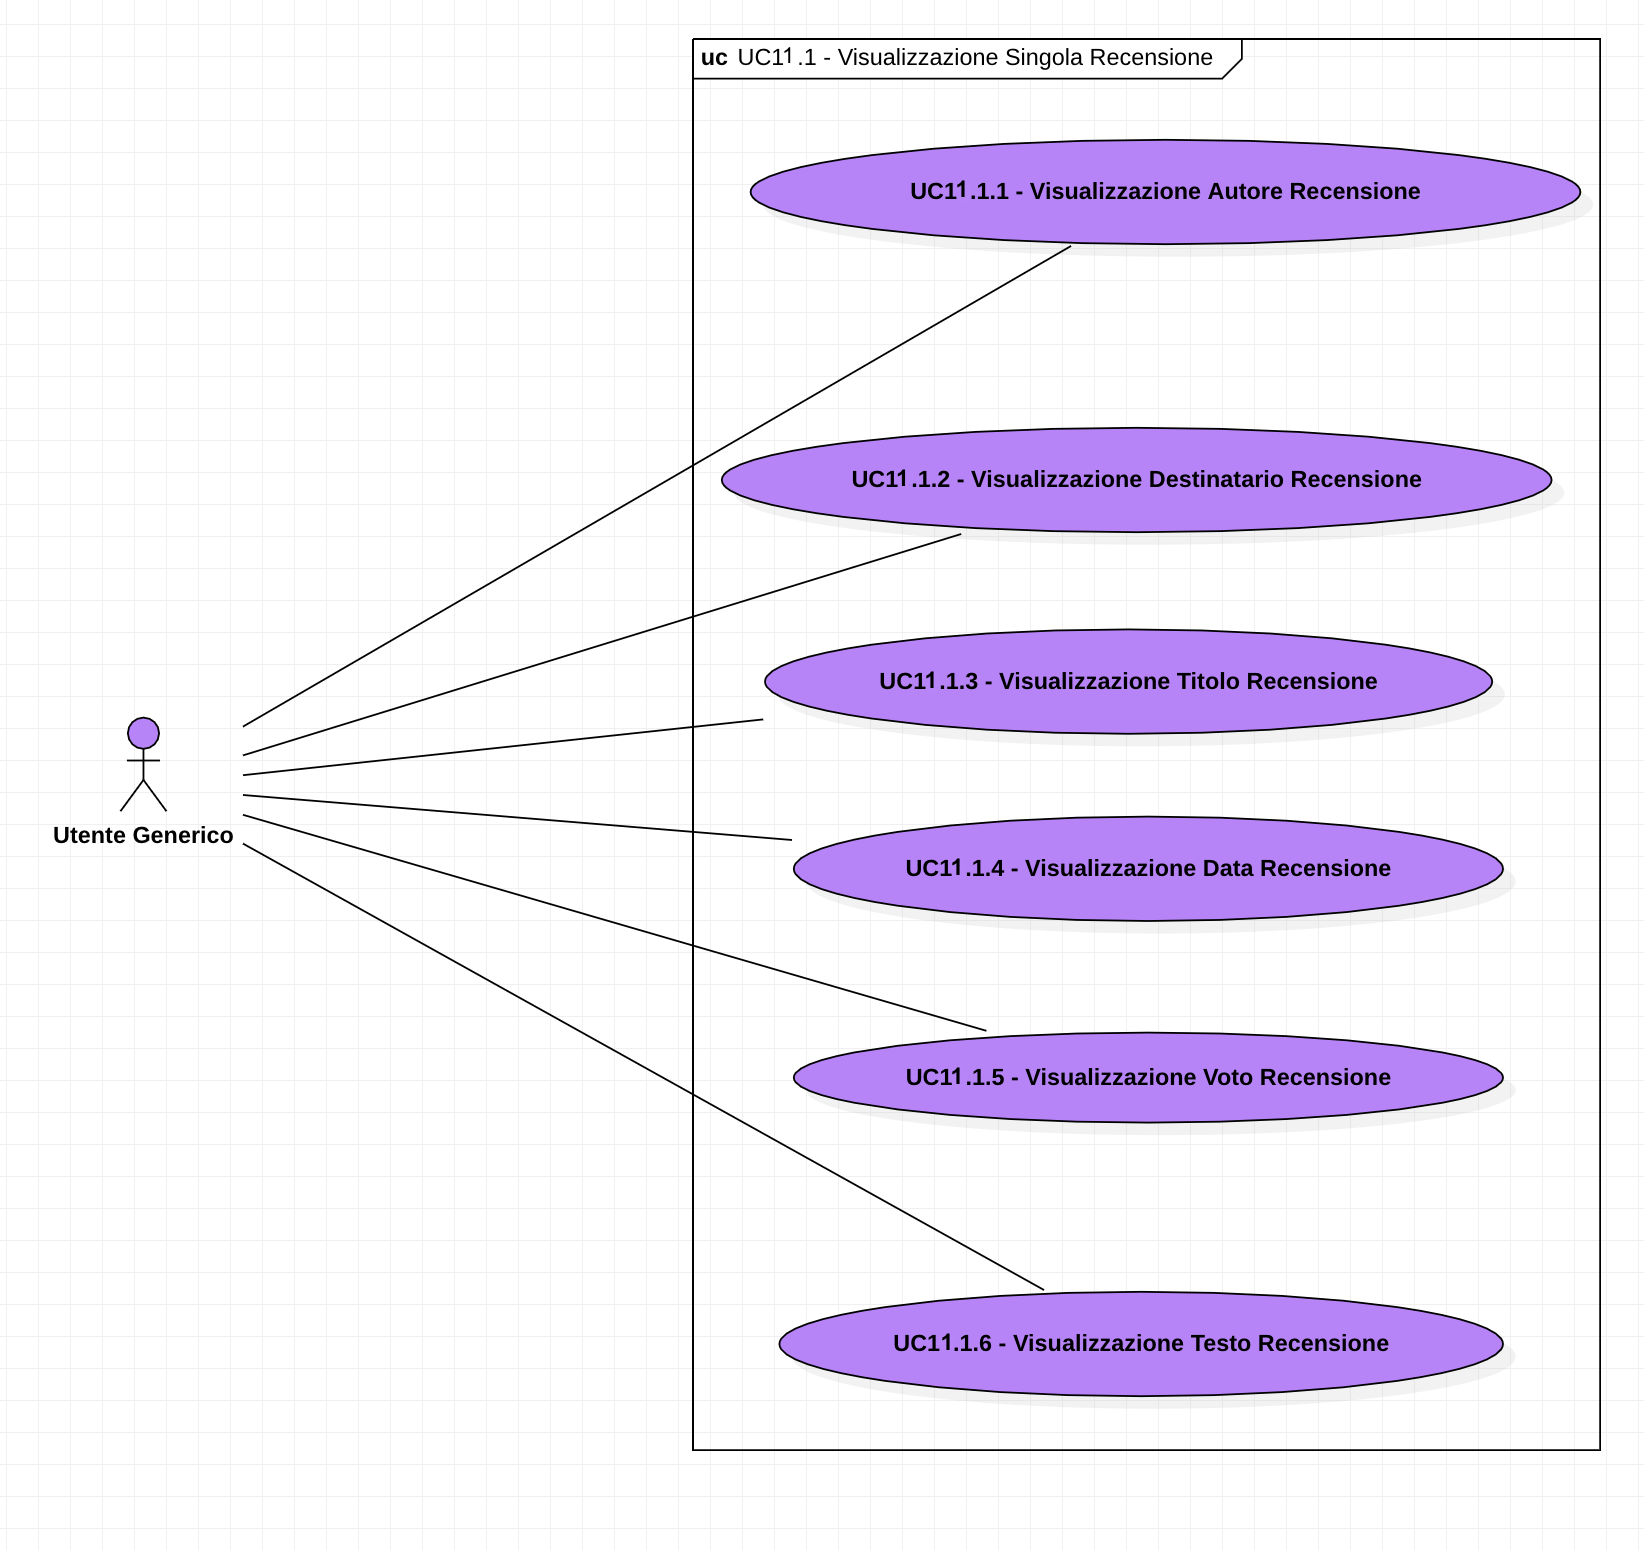
\includegraphics[scale=0.4]{src/img/UC11.1.x.png}
                \caption{UC11.1.1 - UC11.1.6}
            \end{figure}

            \begin{table}[H]
                \centering
                \rowcolors{1}{pari_alt}{dispari_alt}
                \renewcommand{\arraystretch}{1.8}
                \renewcommand\tabularxcolumn[1]{m{#1}}
                \begin{tabularx}{0.9\textwidth} {
                    >{\hsize=.8\hsize\linewidth=\hsize}X
                    >{\hsize=1.2\hsize\linewidth=\hsize}X}
                    \hline
                    \textbf{Attore primario} & Utente generico \\
                    \hline
                    \textbf{Precondizioni} & Si sta visualizzando una lista di recensioni. \\
                    \hline
                    \textbf{Postcondizioni} & Viene visualizzata una singola recensione della lista. \\
                    \hline
                    \textbf{Scenario principale} & Viene visualizzata una recensione appartenente alla lista richiesta dall'utente. \\
                    \hline
                    \textbf{Estensioni} & Se l'operazione non va a buon fine, si verifica \hyperref[UC14]{UC14}. \\
                    \hline
                \end{tabularx}
                \caption{UC11.1}
            \end{table}

        \subsubsection{UC11.1.1 - Visualizzazione Autore Recensione}
        \label{UC11.1.1}

            \begin{table}[H]
                \centering
                \rowcolors{1}{pari_alt}{dispari_alt}
                \renewcommand{\arraystretch}{1.8}
                \renewcommand\tabularxcolumn[1]{m{#1}}
                \begin{tabularx}{0.9\textwidth} {
                    >{\hsize=.8\hsize\linewidth=\hsize}X
                    >{\hsize=1.2\hsize\linewidth=\hsize}X}
                    \hline
                    \textbf{Attore primario} & Utente generico \\
                    \hline
                    \textbf{Precondizioni} & Viene visualizzata una recensione. \\
                    \hline
                    \textbf{Postcondizioni} & Viene visualizzato l'autore della recensione. \\
                    \hline
                    \textbf{Scenario principale} & Viene visualizzato l'autore all'interno della recensione corrispondente. \\
                    \hline
                    \textbf{Estensioni} & Se l'operazione non va a buon fine, si verifica \hyperref[UC14]{UC14}. \\
                    \hline
                \end{tabularx}
                \caption{UC11.1.1}
            \end{table}

        \subsubsection{UC11.1.2 - Visualizzazione Destinatario Recensione}
        \label{UC11.1.2}

            \begin{table}[H]
                \centering
                \rowcolors{1}{pari_alt}{dispari_alt}
                \renewcommand{\arraystretch}{1.8}
                \renewcommand\tabularxcolumn[1]{m{#1}}
                \begin{tabularx}{0.9\textwidth} {
                    >{\hsize=.8\hsize\linewidth=\hsize}X
                    >{\hsize=1.2\hsize\linewidth=\hsize}X}
                    \hline
                    \textbf{Attore primario} & Utente generico \\
                    \hline
                    \textbf{Precondizioni} & Viene visualizzata una recensione. \\
                    \hline
                    \textbf{Postcondizioni} & Viene visualizzato il destinatario della recensione. \\
                    \hline
                    \textbf{Scenario principale} & Viene visualizzato il destinatario all'interno della recensione corrispondente. \\
                    \hline
                    \textbf{Estensioni} & Se l'operazione non va a buon fine, si verifica \hyperref[UC14]{UC14}. \\
                    \hline
                \end{tabularx}
                \caption{UC11.1.2}
            \end{table}

        \subsubsection{UC11.1.3 - Visualizzazione Titolo Recensione}
        \label{UC11.1.3}

            \begin{table}[H]
                \centering
                \rowcolors{1}{pari_alt}{dispari_alt}
                \renewcommand{\arraystretch}{1.8}
                \renewcommand\tabularxcolumn[1]{m{#1}}
                \begin{tabularx}{0.9\textwidth} {
                    >{\hsize=.8\hsize\linewidth=\hsize}X
                    >{\hsize=1.2\hsize\linewidth=\hsize}X}
                    \hline
                    \textbf{Attore primario} & Utente generico \\
                    \hline
                    \textbf{Precondizioni} & Viene visualizzata una recensione. \\
                    \hline
                    \textbf{Postcondizioni} & Viene visualizzato il titolo della recensione. \\
                    \hline
                    \textbf{Scenario principale} & Viene visualizzato il titolo all'interno della recensione corrispondente. \\
                    \hline
                    \textbf{Estensioni} & Se l'operazione non va a buon fine, si verifica \hyperref[UC14]{UC14}. \\
                    \hline
                \end{tabularx}
                \caption{UC11.1.3}
            \end{table}

        \subsubsection{UC11.1.4 - Visualizzazione Data Recensione}
        \label{UC11.1.4}

            \begin{table}[H]
                \centering
                \rowcolors{1}{pari_alt}{dispari_alt}
                \renewcommand{\arraystretch}{1.8}
                \renewcommand\tabularxcolumn[1]{m{#1}}
                \begin{tabularx}{0.9\textwidth} {
                    >{\hsize=.8\hsize\linewidth=\hsize}X
                    >{\hsize=1.2\hsize\linewidth=\hsize}X}
                    \hline
                    \textbf{Attore primario} & Utente generico \\
                    \hline
                    \textbf{Precondizioni} & Viene visualizzata una recensione. \\
                    \hline
                    \textbf{Postcondizioni} & Viene visualizzato la data della recensione. \\
                    \hline
                    \textbf{Scenario principale} & Viene visualizzato la data all'interno della recensione corrispondente. \\
                    \hline
                    \textbf{Estensioni} & Se l'operazione non va a buon fine, si verifica \hyperref[UC14]{UC14}. \\
                    \hline
                \end{tabularx}
                \caption{UC11.1.4}
            \end{table}

        \subsubsection{UC11.1.5 - Visualizzazione Voto Recensione}
        \label{UC11.1.5}

            \begin{table}[H]
                \centering
                \rowcolors{1}{pari_alt}{dispari_alt}
                \renewcommand{\arraystretch}{1.8}
                \renewcommand\tabularxcolumn[1]{m{#1}}
                \begin{tabularx}{0.9\textwidth} {
                    >{\hsize=.8\hsize\linewidth=\hsize}X
                    >{\hsize=1.2\hsize\linewidth=\hsize}X}
                    \hline
                    \textbf{Attore primario} & Utente generico \\
                    \hline
                    \textbf{Precondizioni} & Viene visualizzata una recensione. \\
                    \hline
                    \textbf{Postcondizioni} & Viene visualizzato il voto della recensione. \\
                    \hline
                    \textbf{Scenario principale} & Viene visualizzato il voto all'interno della recensione corrispondente. \\
                    \hline
                    \textbf{Estensioni} & Se l'operazione non va a buon fine, si verifica \hyperref[UC14]{UC14}. \\
                    \hline
                \end{tabularx}
                \caption{UC11.1.5}
            \end{table}

        \subsubsection{UC11.1.6 - Visualizzazione Testo Recensione}
        \label{UC11.1.6}

            \begin{table}[H]
                \centering
                \rowcolors{1}{pari_alt}{dispari_alt}
                \renewcommand{\arraystretch}{1.8}
                \renewcommand\tabularxcolumn[1]{m{#1}}
                \begin{tabularx}{0.9\textwidth} {
                    >{\hsize=.8\hsize\linewidth=\hsize}X
                    >{\hsize=1.2\hsize\linewidth=\hsize}X}
                    \hline
                    \textbf{Attore primario} & Utente generico \\
                    \hline
                    \textbf{Precondizioni} & Viene visualizzata una recensione. \\
                    \hline
                    \textbf{Postcondizioni} & Viene visualizzato il testo della recensione. \\
                    \hline
                    \textbf{Scenario principale} & Viene visualizzato il testo all'interno della recensione corrispondente. \\
                    \hline
                    \textbf{Estensioni} & Se l'operazione non va a buon fine, si verifica \hyperref[UC14]{UC14}. \\
                    \hline
                \end{tabularx}
                \caption{UC11.1.6}
            \end{table}

        \subsubsection{UC12 - Visualizzazione Recensioni Rilasciate}
        \label{UC12}

            \begin{figure}[H]
                \centering
                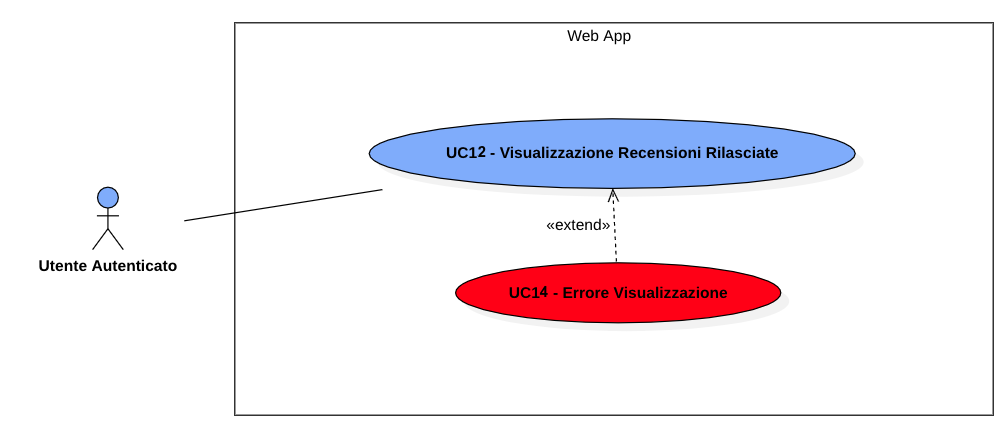
\includegraphics[scale=0.4]{src/img/UC12.png}
                \caption{UC12, UC14}
            \end{figure}

            \begin{table}[H]
                \centering
                \rowcolors{1}{pari_alt}{dispari_alt}
                \renewcommand{\arraystretch}{1.8}
                \renewcommand\tabularxcolumn[1]{m{#1}}
                \begin{tabularx}{0.9\textwidth} {
                    >{\hsize=.8\hsize\linewidth=\hsize}X
                    >{\hsize=1.2\hsize\linewidth=\hsize}X}
                    \hline
                    \textbf{Attore primario} & Utente autenticato \\
                    \hline
                    \textbf{Precondizioni} & L'utente ha effettuato una ricerca delle recensioni rilasciate. \\
                    \hline
                    \textbf{Postcondizioni} & L'utente visualizza le recensioni che ha rilasciato. \\
                    \hline
                    \textbf{Scenario principale} & Viene mostrata la lista di recensioni rilasciate dall'utente. \\
                    \hline
                    \textbf{Estensioni} & Se l'operazione non va a buon fine, si verifica \hyperref[UC14]{UC14}. \\
                    \hline
                \end{tabularx}
                \caption{UC12}
            \end{table}

        \subsubsection{UC13 - Visualizzazione Recensioni Ricevute}
        \label{UC13}

            \begin{figure}[H]
                \centering
                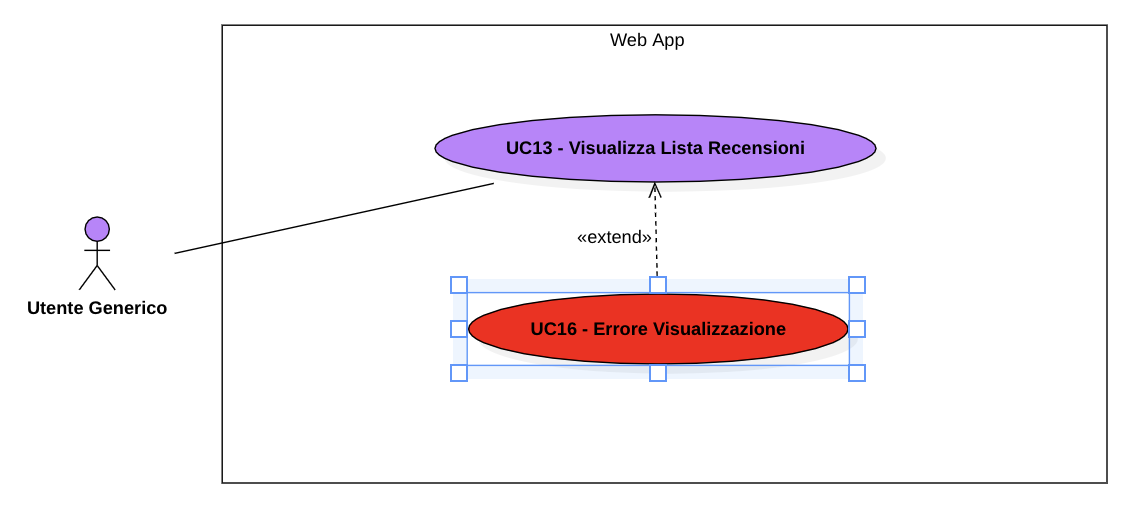
\includegraphics[scale=0.4]{src/img/UC13.png}
                \caption{UC13, UC14}
            \end{figure}

            \begin{table}[H]
                \centering
                \rowcolors{1}{pari_alt}{dispari_alt}
                \renewcommand{\arraystretch}{1.8}
                \renewcommand\tabularxcolumn[1]{m{#1}}
                \begin{tabularx}{0.9\textwidth} {
                    >{\hsize=.8\hsize\linewidth=\hsize}X
                    >{\hsize=1.2\hsize\linewidth=\hsize}X}
                    \hline
                    \textbf{Attore primario} & Utente autenticato \\
                    \hline
                    \textbf{Precondizioni} & L'utente ha effettuato una ricerca delle recensioni ricevute. \\
                    \hline
                    \textbf{Postcondizioni} & L'utente visualizza le recensioni che ha ricevuto. \\
                    \hline
                    \textbf{Scenario principale} & Viene mostrata la lista di recensioni ricevute dall'utente. \\
                    \hline
                    \textbf{Estensioni} & Se l'operazione non va a buon fine, si verifica \hyperref[UC14]{UC14}. \\
                    \hline
                \end{tabularx}
                \caption{UC13}
            \end{table}

        \subsubsection{UC14 - Errore Visualizzazione Recensioni}
        \label{UC14}

            \begin{table}[H]
                \centering
                \rowcolors{1}{pari_alt}{dispari_alt}
                \renewcommand{\arraystretch}{1.8}
                \renewcommand\tabularxcolumn[1]{m{#1}}
                \begin{tabularx}{0.9\textwidth} {
                    >{\hsize=.8\hsize\linewidth=\hsize}X
                    >{\hsize=1.2\hsize\linewidth=\hsize}X}
                    \hline
                    \textbf{Attori primari} & Utente generico, utente autenticato. \\
                    \hline
                    \textbf{Precondizioni} & L'utente richiede la visualizzazione delle recensioni. \\
                    \hline
                    \textbf{Postcondizioni} & La visualizzazione delle recensioni fallita. \\
                    \hline
                    \textbf{Scenario principale} & 
                    \begin{enumerate}
                        \item La visualizzazione delle recensioni fallisce.
                        \item Il sistema mostra un messaggio di errore esplicativo all'utente e si termina l'attuale operazione.
                    \end{enumerate} \\
                    \hline
                \end{tabularx}
                \caption{UC14}
            \end{table}

        \subsubsection{UC15 - Richiesta Lista Recensioni}
        \label{UC15}

            \begin{figure}[H]
                \centering
                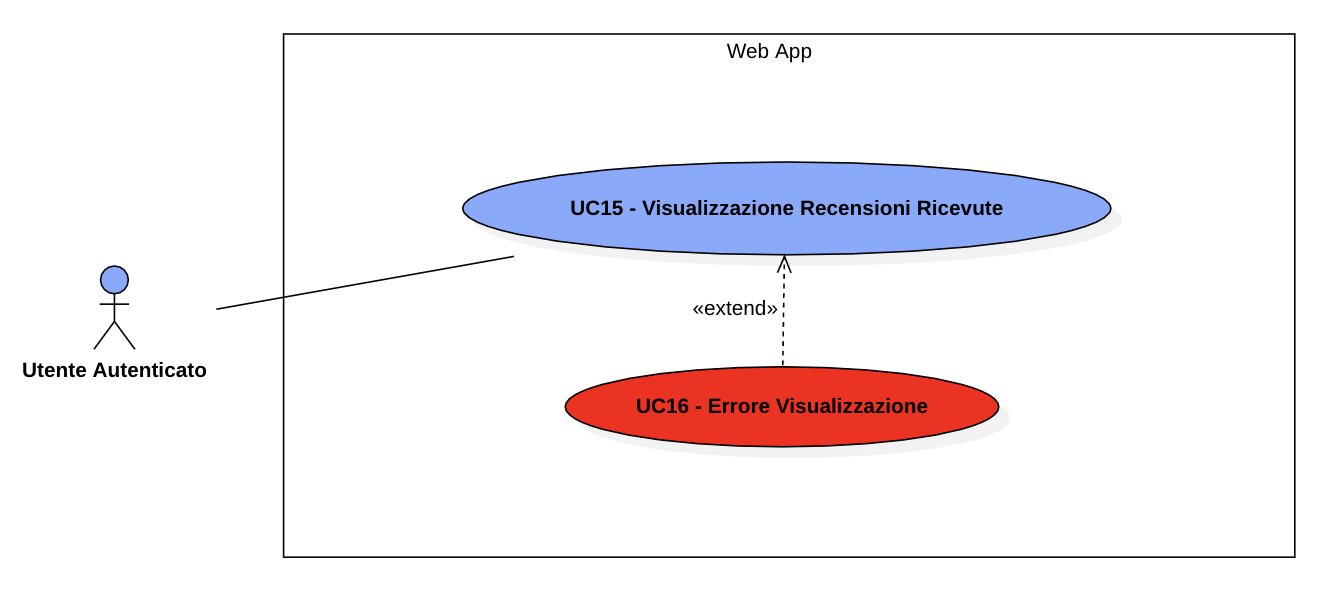
\includegraphics[scale=0.5]{src/img/UC15.png}
                \caption{UC15, UC16}
            \end{figure}

            \begin{table}[H]
                \centering
                \rowcolors{1}{pari_alt}{dispari_alt}
                \renewcommand{\arraystretch}{1.8}
                \renewcommand\tabularxcolumn[1]{m{#1}}
                \begin{tabularx}{0.9\textwidth} {
                    >{\hsize=.8\hsize\linewidth=\hsize}X
                    >{\hsize=1.2\hsize\linewidth=\hsize}X}
                \hline
                \textbf{Attore primario} & Utilizzatore \textit{API} \\
                \hline
                \textbf{Attore secondario} & \textit{Infura} \\
                \hline
                \textbf{Precondizioni} & L'utente deve conoscere l'indirizzo di cui vuole ottenere le recensioni. \\
                \hline
                \textbf{Postcondizioni} & L'utente ottiene una lista di recensioni. \\
                \hline
                \textbf{Scenario principale} &
                    \begin{enumerate}
                        \item L'utente fa una richiesta al \textit{server API REST} per ottenere le recensioni legate all'indirizzo specificato;
                        \item Il server recupera tali recensioni dalla \textit{blockchain};
                        \item Viene restituita la lista di recensioni.
                    \end{enumerate} \\
                \hline
                \textbf{Estensioni} & Se la richiesta fallisce, si verifica \hyperref[UC16]{UC16}. \\
                \hline
                \end{tabularx}
                \caption{UC15}
            \end{table}

        \subsubsection{UC16 - Errore Ottenimento Recensioni}
        \label{UC16}

            \begin{table}[H]
                \centering
                \rowcolors{1}{pari_alt}{dispari_alt}
                \renewcommand{\arraystretch}{1.8}
                \renewcommand\tabularxcolumn[1]{m{#1}}
                \begin{tabularx}{0.9\textwidth} {
                    >{\hsize=.8\hsize\linewidth=\hsize}X
                    >{\hsize=1.2\hsize\linewidth=\hsize}X}
                    \hline
                    \textbf{Attore primario} & Utilizzatore \textit{API} \\
                    \hline
                    \textbf{Attore secondario} & \textit{Infura} \\
                    \hline
                    \textbf{Precondizioni} & L'utente sta tentando di ottenere la lista recensioni. \\
                    \hline
                    \textbf{Postcondizioni} & L'operazione fallisce. \\
                    \hline
                    \textbf{Scenario principale} &
                        \begin{enumerate}
                            \item L'utente tenta di ottenere la lista di recensioni;
                            \item Non esistono delle recensioni legate all'indirizzo cercato;
                            \item Viene mostrato un messaggio di errore.
                        \end{enumerate} \\
                    \hline
                \end{tabularx}
                \caption{UC16}
            \end{table}

        \subsubsection{UC17 - Visualizzazione Lista Pagamenti}
        \label{UC17}

            \begin{figure}[H]
                \centering
                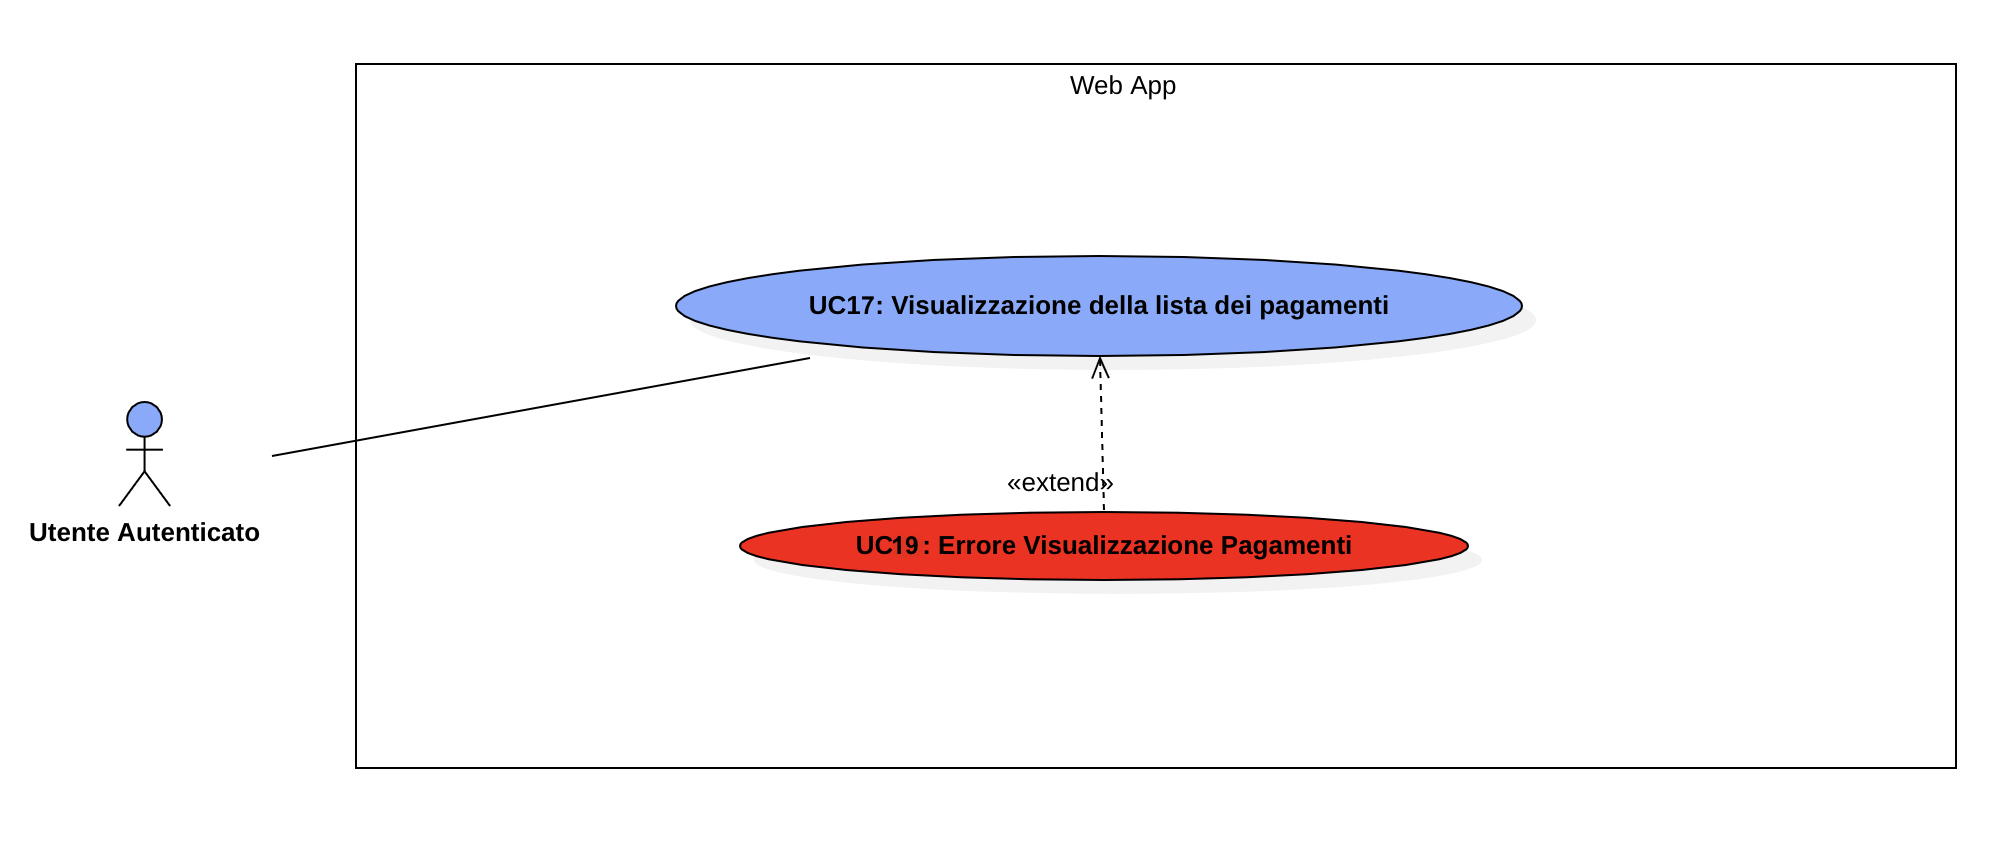
\includegraphics[scale=0.4]{src/img/UC17.png}
                \caption{UC17, UC19}
            \end{figure}

            \begin{table}[H]
                \centering
                \rowcolors{1}{pari_alt}{dispari_alt}
                \renewcommand{\arraystretch}{1.8}
                \renewcommand\tabularxcolumn[1]{m{#1}}
                \begin{tabularx}{0.9\textwidth} {
                    >{\hsize=.8\hsize\linewidth=\hsize}X
                    >{\hsize=1.2\hsize\linewidth=\hsize}X}
                    \hline
                    \textbf{Attore primario} & Utente autenticato \\
                    \hline
                    \textbf{Precondizioni} & L'utente ha effettuato almeno un pagamento. \\
                    \hline
                    \textbf{Postcondizioni} & L'utente visualizza la lista di tutti i suoi pagamenti. \\
                    \hline
                    \textbf{Scenario principale} & Viene visualizzata la lista dei pagamenti. \\
                    \hline
                    \textbf{Estensioni} & Se l'operazione non va a buon fine, si verifica \hyperref[UC18]{UC18}. \\
                    \hline
                \end{tabularx}
                \caption{UC17}
            \end{table}

        \subsubsection{UC17.1 - Visualizzazione Singolo Pagamento}
        \label{UC17.1}

            \begin{figure}[H]
                \centering
                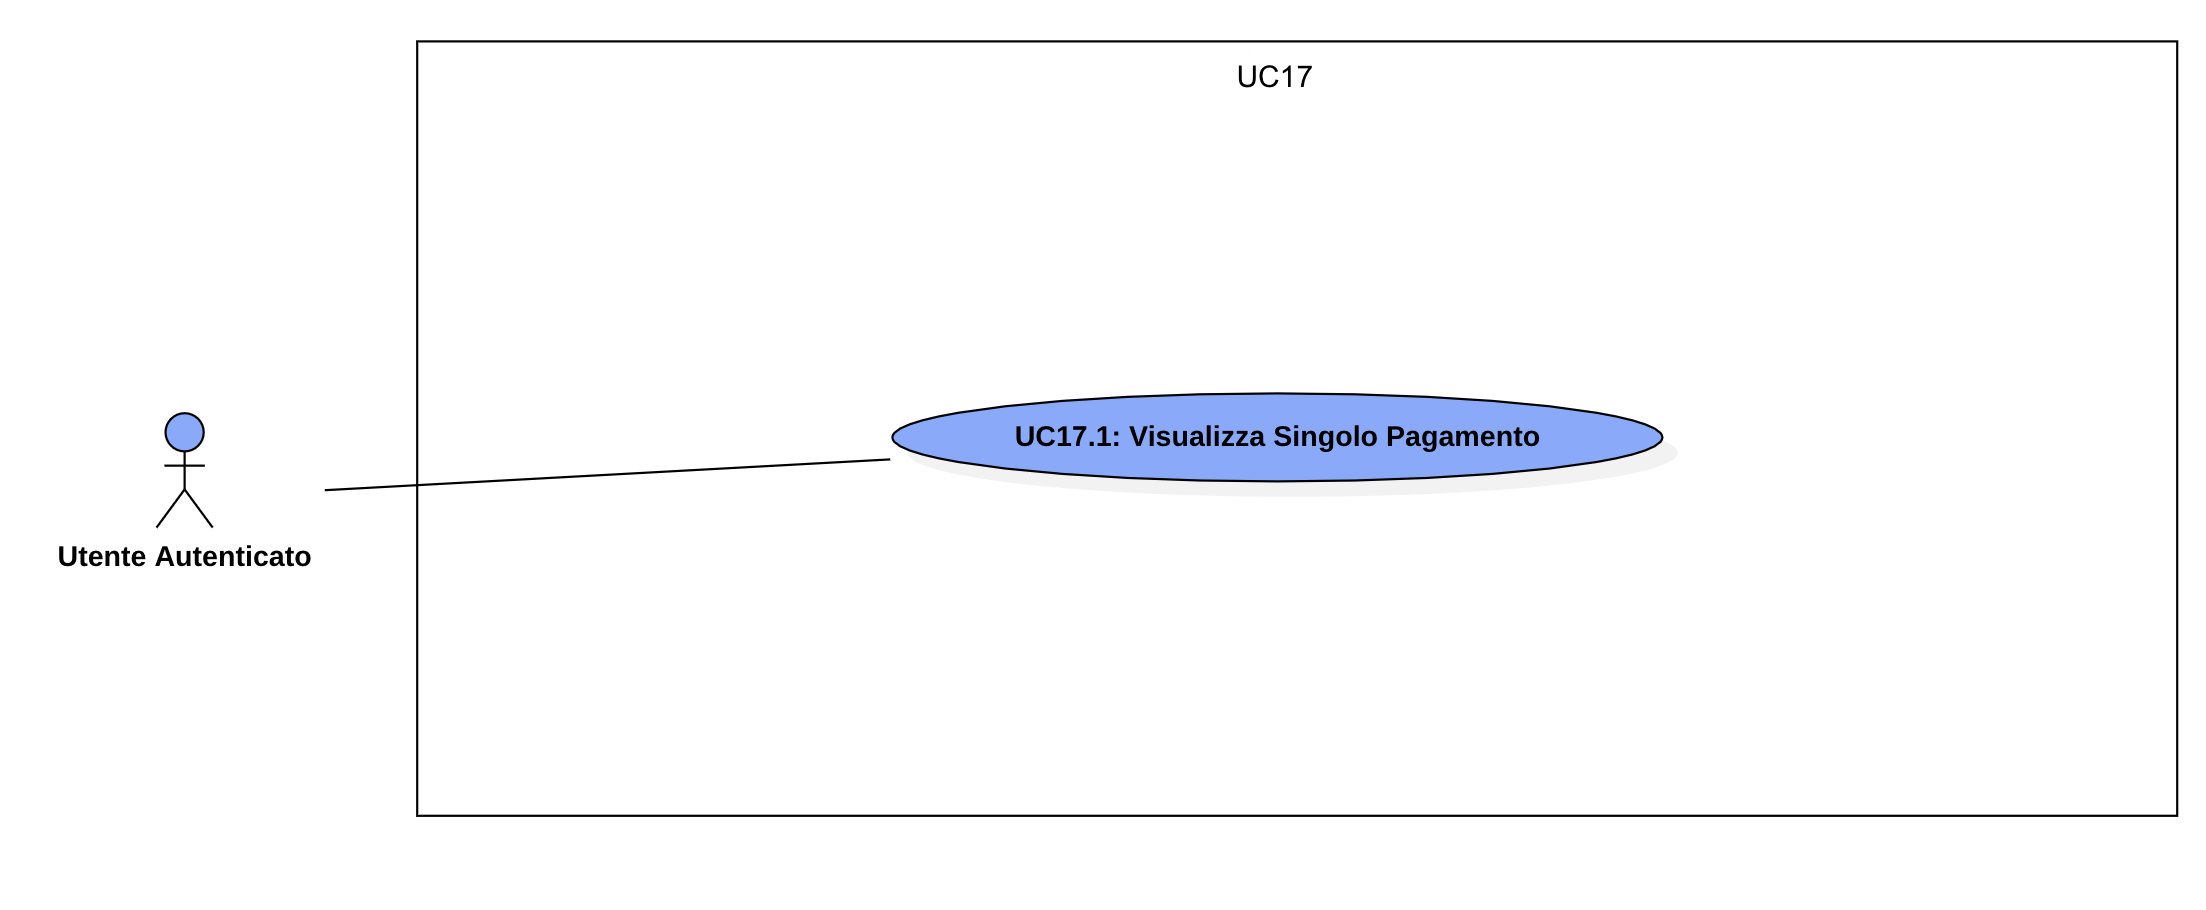
\includegraphics[scale=0.4]{src/img/UC17.1.png}
                \caption{UC17.1}
                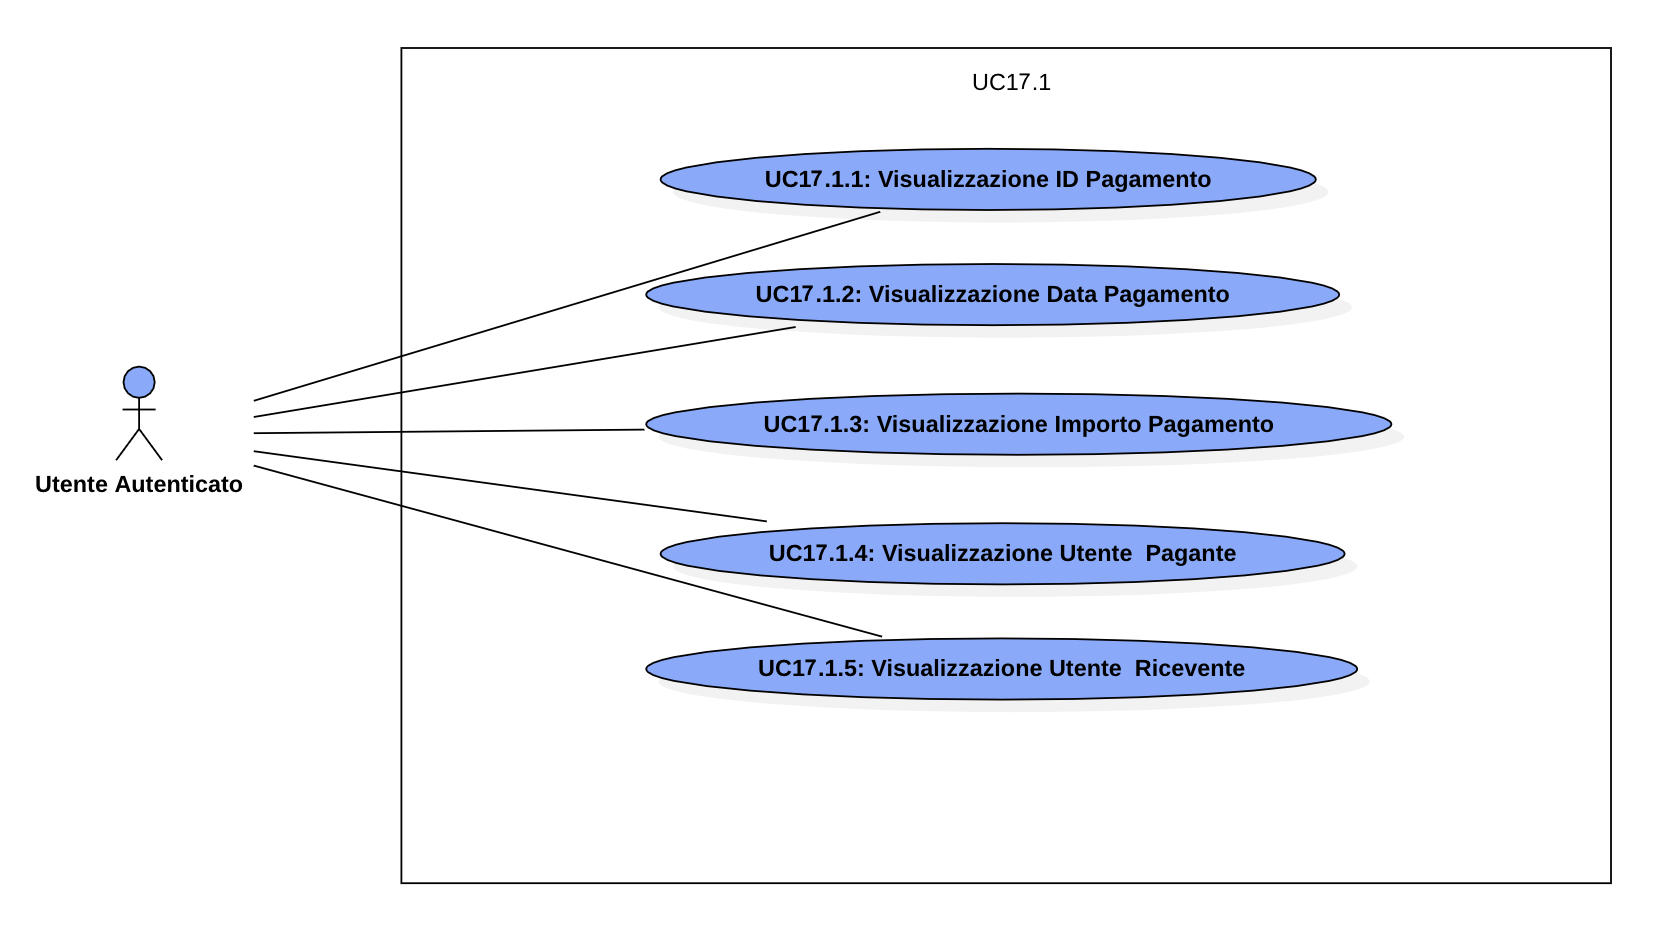
\includegraphics[scale=0.4]{src/img/UC17.1.x.png}
                \caption{UC17.1.1 - UC17.1.5}
            \end{figure}

            \begin{table}[H]
                \centering
                \rowcolors{1}{pari_alt}{dispari_alt}
                \renewcommand{\arraystretch}{1.8}
                \renewcommand\tabularxcolumn[1]{m{#1}}
                \begin{tabularx}{0.9\textwidth} {
                    >{\hsize=.8\hsize\linewidth=\hsize}X
                    >{\hsize=1.2\hsize\linewidth=\hsize}X}
                    \hline
                    \textbf{Attore primario} & Utente autenticato \\
                    \hline
                    \textbf{Precondizioni} & L'utente ha selezionato un pagamento dalla lista. \\
                    \hline
                    \textbf{Postcondizioni} & L'utente visualizza il singolo pagamento selezionato. \\
                    \hline
                    \textbf{Scenario principale} & Visualizzazione del singolo pagamento. \\
                    \hline
                    \textbf{Estensioni} & Se l'operazione non va a buon fine, si verifica \hyperref[UC18]{UC18}. \\
                    \hline
                \end{tabularx}
                \caption{UC17.1}
            \end{table}

        \subsubsection{UC17.1.1 - Visualizzazione ID Pagamento}
        \label{UC17.1.1}

            \begin{table}[H]
                \centering
                \rowcolors{1}{pari_alt}{dispari_alt}
                \renewcommand{\arraystretch}{1.8}
                \renewcommand\tabularxcolumn[1]{m{#1}}
                \begin{tabularx}{0.9\textwidth} {
                    >{\hsize=.8\hsize\linewidth=\hsize}X
                    >{\hsize=1.2\hsize\linewidth=\hsize}X}
                    \hline
                    \textbf{Attore primario} & Utente autenticato \\
                    \hline
                    \textbf{Precondizioni} & L'utente ha visualizzato un singolo pagamento della lista. \\
                    \hline
                    \textbf{Postcondizioni} & L'utente visualizza l'ID del pagamento. \\
                    \hline
                    \textbf{Scenario principale} & Visualizzazione ID del singolo pagamento. \\
                    \hline
                    \textbf{Estensioni} & Se l'operazione non va a buon fine, si verifica \hyperref[UC18]{UC18}. \\
                    \hline
                \end{tabularx}
                \caption{UC17.1.1}
            \end{table}

        \subsubsection{UC17.1.2 - Visualizzazione Data Pagamento}
        \label{UC17.1.2}

            \begin{table}[H]
                \centering
                \rowcolors{1}{pari_alt}{dispari_alt}
                \renewcommand{\arraystretch}{1.8}
                \renewcommand\tabularxcolumn[1]{m{#1}}
                \begin{tabularx}{0.9\textwidth} {
                    >{\hsize=.8\hsize\linewidth=\hsize}X
                    >{\hsize=1.2\hsize\linewidth=\hsize}X}
                    \hline
                    \textbf{Attore primario} & Utente autenticato \\
                    \hline
                    \textbf{Precondizioni} & L'utente ha visualizzato un singolo pagamento della lista. \\
                    \hline
                    \textbf{Postcondizioni} & L'utente visualizza la data del pagamento. \\
                    \hline
                    \textbf{Scenario principale} & Visualizzazione della data del singolo pagamento. \\
                    \hline
                    \textbf{Estensioni} & Se l'operazione non va a buon fine, si verifica \hyperref[UC18]{UC18}. \\
                    \hline
                \end{tabularx}
                \caption{UC17.1.2}
            \end{table}

        \subsubsection{UC17.1.3 - Visualizzazione Importo Pagamento}
        \label{UC17.1.3}

            \begin{table}[H]
                \centering
                \rowcolors{1}{pari_alt}{dispari_alt}
                \renewcommand{\arraystretch}{1.8}
                \renewcommand\tabularxcolumn[1]{m{#1}}
                \begin{tabularx}{0.9\textwidth} {
                    >{\hsize=.8\hsize\linewidth=\hsize}X
                    >{\hsize=1.2\hsize\linewidth=\hsize}X}
                    \hline
                    \textbf{Attore primario} & Utente autenticato \\
                    \hline
                    \textbf{Precondizioni} & L'utente ha visualizzato un singolo pagamento della lista. \\
                    \hline
                    \textbf{Postcondizioni} & L'utente visualizza l'importo del pagamento. \\
                    \hline
                    \textbf{Scenario principale} & Visualizzazione importo del singolo pagamento. \\
                    \hline
                    \textbf{Estensioni} & Se l'operazione non va a buon fine, si verifica \hyperref[UC18]{UC18}. \\
                    \hline
                \end{tabularx}
                \caption{UC17.1.3}
            \end{table}
        
        \subsubsection{UC17.1.4 - Visualizzazione Utente Pagante Pagamento}
        \label{UC17.1.4}

            \begin{table}[H]
                \centering
                \rowcolors{1}{pari_alt}{dispari_alt}
                \renewcommand{\arraystretch}{1.8}
                \renewcommand\tabularxcolumn[1]{m{#1}}
                \begin{tabularx}{0.9\textwidth} {
                    >{\hsize=.8\hsize\linewidth=\hsize}X
                    >{\hsize=1.2\hsize\linewidth=\hsize}X}
                    \hline
                    \textbf{Attore primario} & Utente autenticato \\
                    \hline
                    \textbf{Precondizioni} & L'utente ha visualizzato un singolo pagamento della lista. \\
                    \hline
                    \textbf{Postcondizioni} & L'utente visualizza l'utente pagante del pagamento. \\
                    \hline
                    \textbf{Scenario principale} & Visualizzazione utente pagante del singolo pagamento. \\
                    \hline
                    \textbf{Estensioni} & Se l'operazione non va a buon fine, si verifica \hyperref[UC18]{UC18}. \\
                    \hline
                \end{tabularx}
                \caption{UC17.1.4}
            \end{table}

        \subsubsection{UC17.1.5 - Visualizzazione Utente Ricevente Pagamento}
        \label{UC17.1.5}

            \begin{table}[H]
                \centering
                \rowcolors{1}{pari_alt}{dispari_alt}
                \renewcommand{\arraystretch}{1.8}
                \renewcommand\tabularxcolumn[1]{m{#1}}
                \begin{tabularx}{0.9\textwidth} {
                    >{\hsize=.8\hsize\linewidth=\hsize}X
                    >{\hsize=1.2\hsize\linewidth=\hsize}X}
                    \hline
                    \textbf{Attore primario} & Utente autenticato \\
                    \hline
                    \textbf{Precondizioni} & L'utente ha visualizzato un singolo pagamento della lista. \\
                    \hline
                    \textbf{Postcondizioni} & L'utente visualizza l'utente ricevente del pagamento. \\
                    \hline
                    \textbf{Scenario principale} & Visualizzazione utente ricevente del singolo pagamento. \\
                    \hline
                    \textbf{Estensioni} & Se l'operazione non va a buon fine, si verifica \hyperref[UC18]{UC18}. \\
                    \hline
                \end{tabularx}
                \caption{UC17.1.5}
            \end{table}

        \subsubsection{UC18 - Errore Visualizzazione Pagamenti}
        \label{UC18}

            \begin{table}[H]
                \centering
                \rowcolors{1}{pari_alt}{dispari_alt}
                \renewcommand{\arraystretch}{1.8}
                \renewcommand\tabularxcolumn[1]{m{#1}}
                \begin{tabularx}{0.9\textwidth} {
                    >{\hsize=.8\hsize\linewidth=\hsize}X
                    >{\hsize=1.2\hsize\linewidth=\hsize}X}
                    \hline
                    \textbf{Attori primari} & Utente autenticato. \\
                    \hline
                    \textbf{Precondizioni} & L'utente richiede la visualizzazione della lista dei pagamenti che ha effettuato. \\
                    \hline
                    \textbf{Postcondizioni} & La visualizzazione dei pagamenti fallita. \\
                    \hline
                    \textbf{Scenario principale} & 
                    \begin{enumerate}
                        \item La visualizzazione dei pagamenti fallisce.
                        \item Il sistema mostra un messaggio di errore all'utente su circa il motivo.
                        \item Vengono mostrati consigli sulla risoluzione del problema e si termina l'attuale operazione.
                    \end{enumerate} \\
                    \hline
                \end{tabularx}
                \caption{UC18}
            \end{table}

            \subsubsection{UC19 - Ordinamento Lista Recensioni}
            \label{UC19}

            \begin{figure}[H]
                \centering
                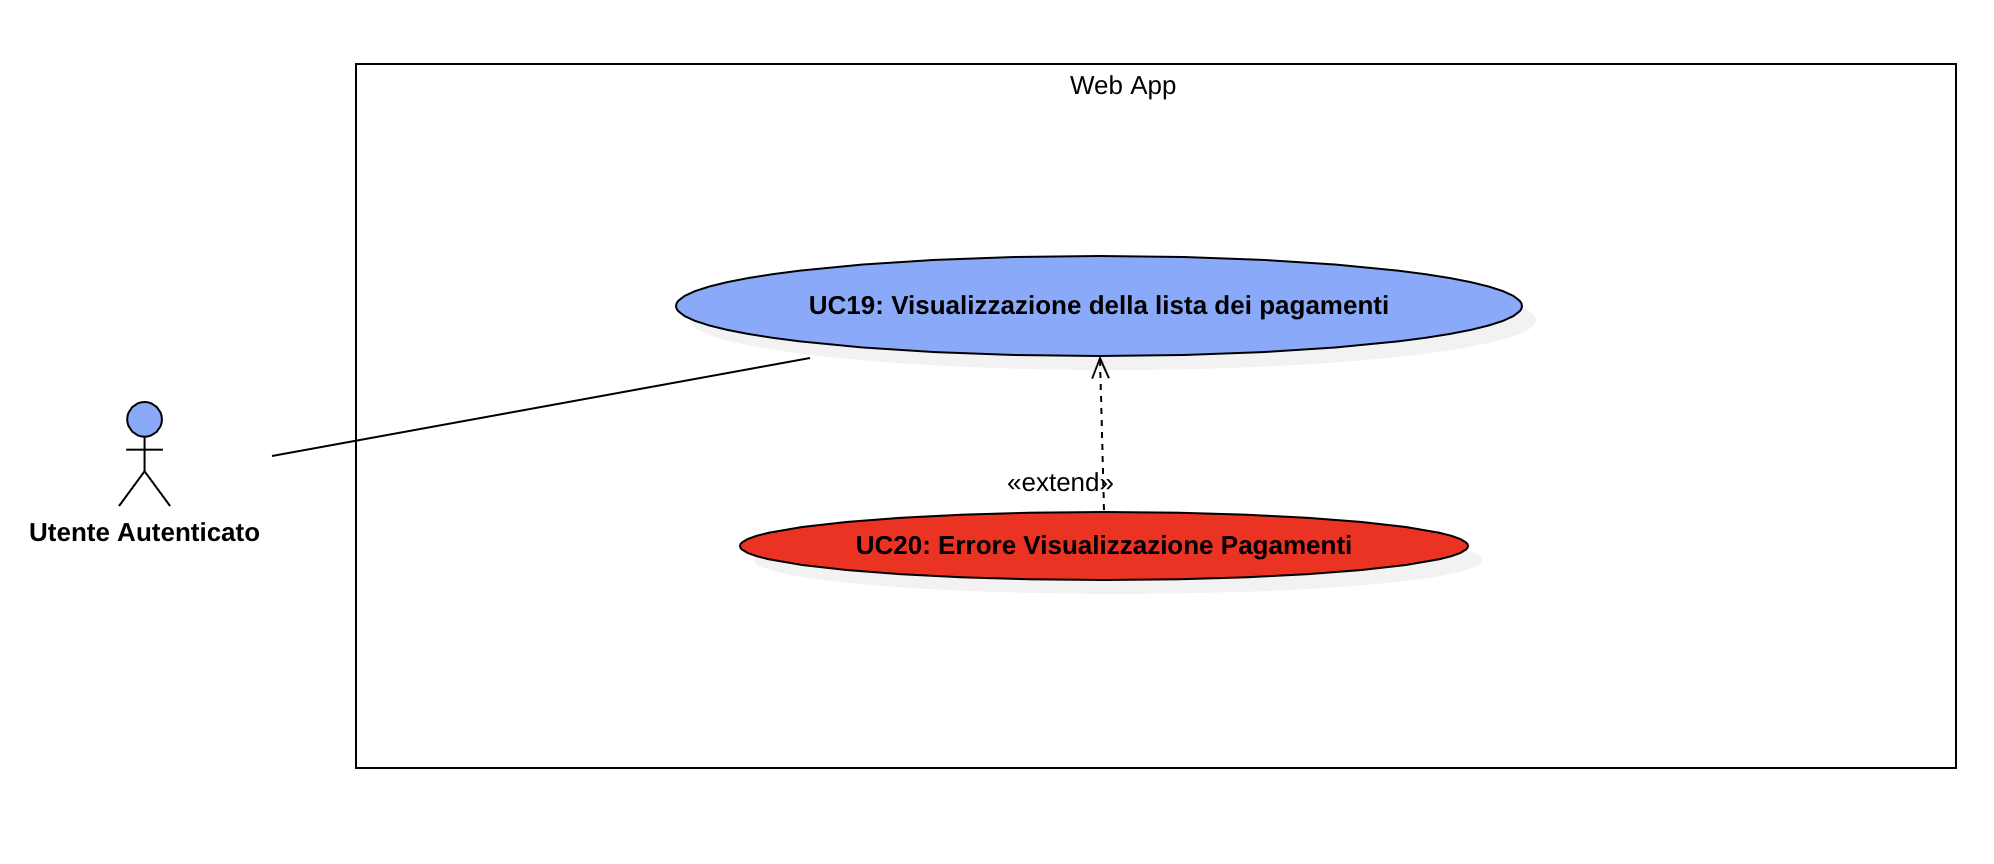
\includegraphics[scale=0.4]{src/img/UC19.png}
                \caption{UC19, UC20, UC21}
            \end{figure}

            \begin{table}[H]
                \centering
                \rowcolors{1}{pari_alt}{dispari_alt}
                \renewcommand{\arraystretch}{1.8}
                \renewcommand\tabularxcolumn[1]{m{#1}}
                \begin{tabularx}{0.9\textwidth} {
                    >{\hsize=.8\hsize\linewidth=\hsize}X
                    >{\hsize=1.2\hsize\linewidth=\hsize}X}
                    \hline
                    \textbf{Attore primario} & Utente generico \\
                    \hline
                    \textbf{Precondizioni} & L'utente ha effettuato una ricerca delle recensioni, che è andata a buon fine. \\
                    \hline
                    \textbf{Postcondizioni} & L'utente visualizza la lista di tutte le recensioni ordinate. \\
                    \hline
                    \textbf{Scenario principale} & Viene visualizzata la lista delle recensioni in ordine. \\
                    \hline
                    \textbf{Estensioni} & Se l'operazione non va a buon fine, si verifica \hyperref[UC14]{UC14}. \\
                    \hline
                \end{tabularx}
                \caption{UC19}
            \end{table}

        \subsubsection{UC20 - Ordinamento Lista Recensioni dal meno recente}
        \label{UC20}

            \begin{table}[H]
                \centering
                \rowcolors{1}{pari_alt}{dispari_alt}
                \renewcommand{\arraystretch}{1.8}
                \renewcommand\tabularxcolumn[1]{m{#1}}
                \begin{tabularx}{0.9\textwidth} {
                    >{\hsize=.8\hsize\linewidth=\hsize}X
                    >{\hsize=1.2\hsize\linewidth=\hsize}X}
                    \hline
                    \textbf{Attore primario} & Utente generico \\
                    \hline
                    \textbf{Precondizioni} & L'utente ha effettuato una ricerca delle recensioni, che è andata a buon fine. \\
                    \hline
                    \textbf{Postcondizioni} & L'utente visualizza la lista di tutte le recensioni, ordinati dal più recente. \\
                    \hline
                    \textbf{Scenario principale} & Viene visualizzata la lista delle recensioni, ordinate dal più recente. \\
                    \hline
                    \textbf{Estensioni} & Se l'operazione non va a buon fine, si verifica \hyperref[UC14]{UC14}. \\
                    \hline
                \end{tabularx}
                \caption{UC20}
            \end{table}

            \subsubsection{UC21 - Ordinamento Lista Recensioni dal più recente}
            \label{UC21}

                \begin{table}[H]
                    \centering
                    \rowcolors{1}{pari_alt}{dispari_alt}
                    \renewcommand{\arraystretch}{1.8}
                    \renewcommand\tabularxcolumn[1]{m{#1}}
                    \begin{tabularx}{0.9\textwidth} {
                        >{\hsize=.8\hsize\linewidth=\hsize}X
                        >{\hsize=1.2\hsize\linewidth=\hsize}X}
                        \hline
                        \textbf{Attore primario} & Utente generico \\
                        \hline
                        \textbf{Precondizioni} & L'utente ha effettuato una ricerca delle recensioni, che è andata a buon fine. \\
                        \hline
                        \textbf{Postcondizioni} & L'utente visualizza la lista di tutte le recensioni, ordinati dal più recente. \\
                        \hline
                        \textbf{Scenario principale} & Viene visualizzata la lista delle recensioni, ordinate dal più recente. \\
                        \hline
                        \textbf{Estensioni} & Se l'operazione non va a buon fine, si verifica \hyperref[UC14]{UC14}. \\
                        \hline
                    \end{tabularx}
                    \caption{UC21}
                \end{table}

                \subsubsection{UC22 - Visualizzazione Lista Pagamenti ordinati cronologicamente}
            \label{UC22}

            \begin{figure}[H]
                \centering
                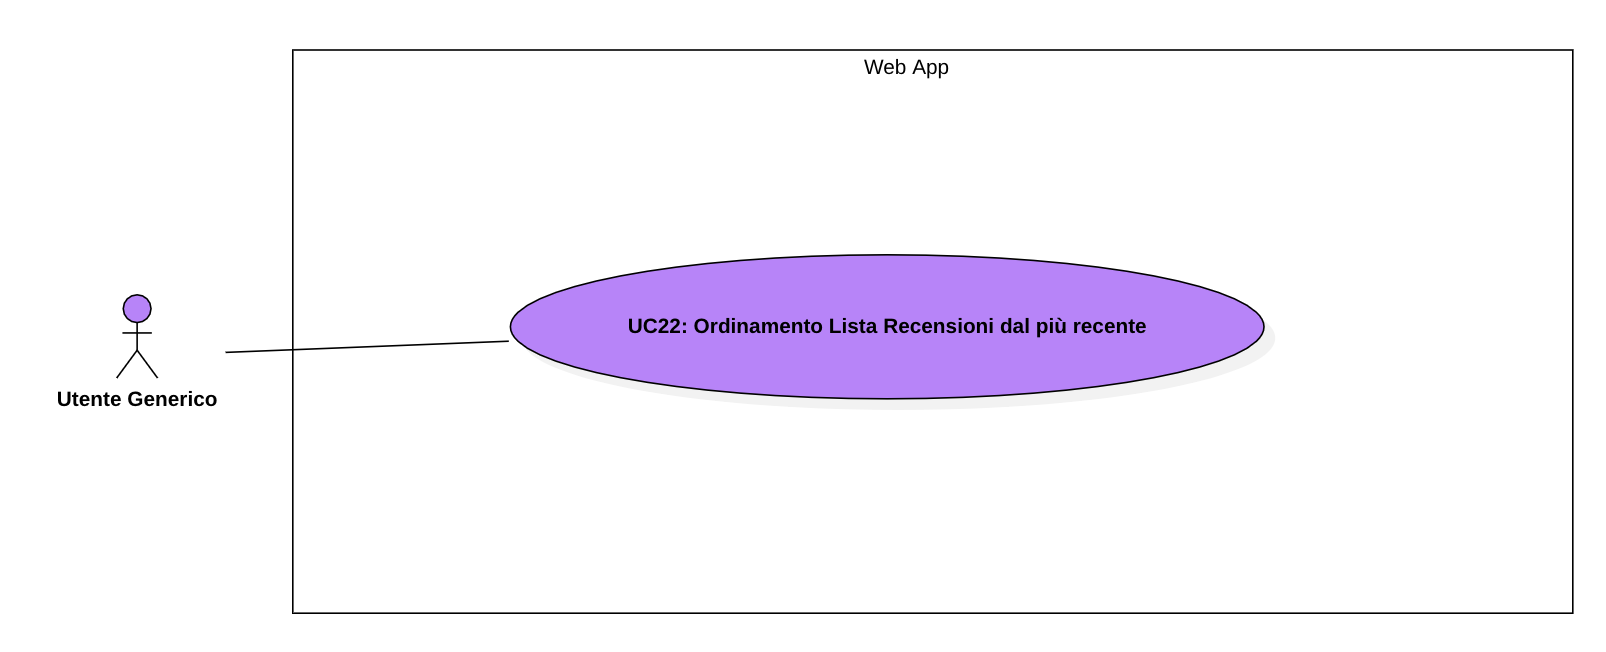
\includegraphics[scale=0.4]{src/img/UC22.png}
                \caption{UC22, UC23, UC24}
            \end{figure}

                \begin{table}[H]
                    \centering
                    \rowcolors{1}{pari_alt}{dispari_alt}
                    \renewcommand{\arraystretch}{1.8}
                    \renewcommand\tabularxcolumn[1]{m{#1}}
                    \begin{tabularx}{0.9\textwidth} {
                        >{\hsize=.8\hsize\linewidth=\hsize}X
                        >{\hsize=1.2\hsize\linewidth=\hsize}X}
                        \hline
                        \textbf{Attore primario} & Utente autenticato \\
                        \hline
                        \textbf{Precondizioni} & L'utente ha effettuato almeno un pagamento. \\
                        \hline
                        \textbf{Postcondizioni} & L'utente visualizza la lista di tutti i suoi pagamenti ordinati. \\
                        \hline
                        \textbf{Scenario principale} & Viene visualizzata la lista dei pagamenti in ordine. \\
                        \hline
                        \textbf{Estensioni} & Se l'operazione non va a buon fine, si verifica \hyperref[UC18]{UC18}. \\
                        \hline
                    \end{tabularx}
                    \caption{UC22}
                \end{table}


            \subsubsection{UC23 - Visualizzazione Lista Pagamenti ordinati dal meno recente}
            \label{UC23}


                \begin{table}[H]
                    \centering
                    \rowcolors{1}{pari_alt}{dispari_alt}
                    \renewcommand{\arraystretch}{1.8}
                    \renewcommand\tabularxcolumn[1]{m{#1}}
                    \begin{tabularx}{0.9\textwidth} {
                        >{\hsize=.8\hsize\linewidth=\hsize}X
                        >{\hsize=1.2\hsize\linewidth=\hsize}X}
                        \hline
                        \textbf{Attore primario} & Utente autenticato \\
                        \hline
                        \textbf{Precondizioni} & L'utente ha effettuato almeno un pagamento. \\
                        \hline
                        \textbf{Postcondizioni} & L'utente visualizza la lista di tutti i suoi pagamenti, ordinati dal meno recente. \\
                        \hline
                        \textbf{Scenario principale} & Viene visualizzata la lista dei pagamenti in ordine cronologico. \\
                        \hline
                        \textbf{Estensioni} & Se l'operazione non va a buon fine, si verifica \hyperref[UC18]{UC18}. \\
                        \hline
                    \end{tabularx}
                    \caption{UC23}
                \end{table}

        \subsubsection{UC24 - Visualizzazione Lista Pagamenti ordinati dal più recente}
        \label{UC24}

            \begin{table}[H]
                \centering
                \rowcolors{1}{pari_alt}{dispari_alt}
                \renewcommand{\arraystretch}{1.8}
                \renewcommand\tabularxcolumn[1]{m{#1}}
                \begin{tabularx}{0.9\textwidth} {
                    >{\hsize=.8\hsize\linewidth=\hsize}X
                    >{\hsize=1.2\hsize\linewidth=\hsize}X}
                    \hline
                    \textbf{Attore primario} & Utente autenticato \\
                    \hline
                    \textbf{Precondizioni} & L'utente ha effettuato almeno un pagamento. \\
                    \hline
                    \textbf{Postcondizioni} & L'utente visualizza la lista di tutti i suoi pagamenti, ordinati dal più recente. \\
                    \hline
                    \textbf{Scenario principale} & Viene visualizzata la lista dei pagamenti ordinati dal più recente. \\
                    \hline
                    \textbf{Estensioni} & Se l'operazione non va a buon fine, si verifica \hyperref[UC18]{UC18}. \\
                    \hline
                \end{tabularx}
                \caption{UC24}
            \end{table}

            \subsubsection{UC25 - Visualizzazione Lista Pagamenti ordinati in base all'importo}
        \label{UC25}

        \begin{figure}[H]
            \centering
            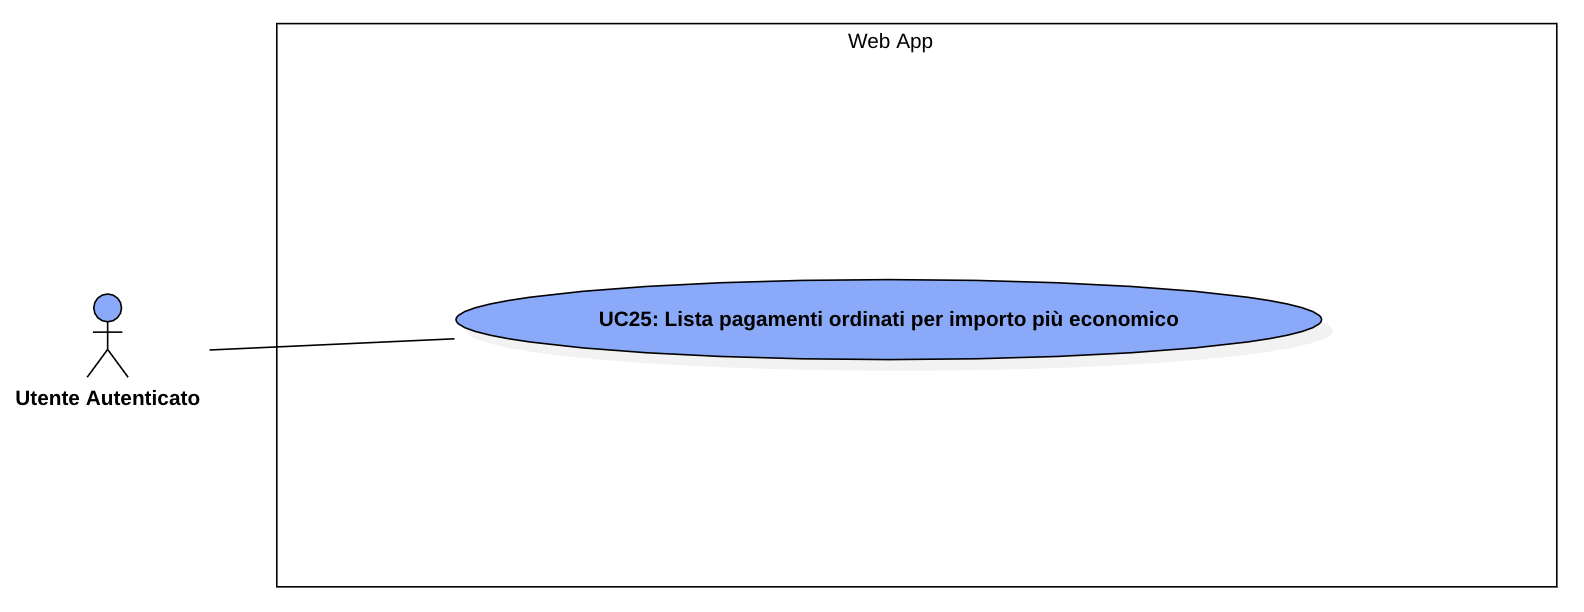
\includegraphics[scale=0.4]{src/img/UC25.png}
            \caption{UC25, UC16, UC27}
        \end{figure}

            \begin{table}[H]
                \centering
                \rowcolors{1}{pari_alt}{dispari_alt}
                \renewcommand{\arraystretch}{1.8}
                \renewcommand\tabularxcolumn[1]{m{#1}}
                \begin{tabularx}{0.9\textwidth} {
                    >{\hsize=.8\hsize\linewidth=\hsize}X
                    >{\hsize=1.2\hsize\linewidth=\hsize}X}
                    \hline
                    \textbf{Attore primario} & Utente autenticato \\
                    \hline
                    \textbf{Precondizioni} & L'utente ha effettuato almeno un pagamento. \\
                    \hline
                    \textbf{Postcondizioni} & L'utente visualizza la lista di tutti i suoi pagamenti, ordinati per importo più economico. \\
                    \hline
                    \textbf{Scenario principale} & Viene visualizzata la lista dei pagamenti in ordine. \\
                    \hline
                    \textbf{Estensioni} & Se l'operazione non va a buon fine, si verifica \hyperref[UC18]{UC18}. \\
                    \hline
                \end{tabularx}
                \caption{UC25}
            \end{table}

        \subsubsection{UC26 - Visualizzazione Lista Pagamenti ordinati per importo più economico}
        \label{UC26}


            \begin{table}[H]
                \centering
                \rowcolors{1}{pari_alt}{dispari_alt}
                \renewcommand{\arraystretch}{1.8}
                \renewcommand\tabularxcolumn[1]{m{#1}}
                \begin{tabularx}{0.9\textwidth} {
                    >{\hsize=.8\hsize\linewidth=\hsize}X
                    >{\hsize=1.2\hsize\linewidth=\hsize}X}
                    \hline
                    \textbf{Attore primario} & Utente autenticato \\
                    \hline
                    \textbf{Precondizioni} & L'utente ha effettuato almeno un pagamento. \\
                    \hline
                    \textbf{Postcondizioni} & L'utente visualizza la lista di tutti i suoi pagamenti, ordinati per importo più economico. \\
                    \hline
                    \textbf{Scenario principale} & Viene visualizzata la lista dei pagamenti in ordine dal più economico. \\
                    \hline
                    \textbf{Estensioni} & Se l'operazione non va a buon fine, si verifica \hyperref[UC18]{UC18}. \\
                    \hline
                \end{tabularx}
                \caption{UC26}
            \end{table}

        \subsubsection{UC27 - Visualizzazione Lista Pagamenti ordinati per importo meno economico}
        \label{UC27}

            \begin{table}[H]
                \centering
                \rowcolors{1}{pari_alt}{dispari_alt}
                \renewcommand{\arraystretch}{1.8}
                \renewcommand\tabularxcolumn[1]{m{#1}}
                \begin{tabularx}{0.9\textwidth} {
                    >{\hsize=.8\hsize\linewidth=\hsize}X
                    >{\hsize=1.2\hsize\linewidth=\hsize}X}
                    \hline
                    \textbf{Attore primario} & Utente autenticato \\
                    \hline
                    \textbf{Precondizioni} & L'utente ha effettuato almeno un pagamento. \\
                    \hline
                    \textbf{Postcondizioni} & L'utente visualizza la lista di tutti i suoi pagamenti, ordinati per importo meno economico. \\
                    \hline
                    \textbf{Scenario principale} & Viene visualizzata la lista dei pagamenti in ordine dal meno economico. \\
                    \hline
                    \textbf{Estensioni} & Se l'operazione non va a buon fine, si verifica \hyperref[UC18]{UC18}. \\
                    \hline
                \end{tabularx}
                \caption{UC27}
            \end{table}

\pagebreak